\chapter{Ефекти впливу гамма--опромінення та ультразвукового навантаження при кімнатних температурах
на структури Al$-n-n^+$--Si---Al з контактом Шотки\label{Ch_GammaSD}}

Як відомо, структури метал--напівпровідник є основою для створення різноманітних польових транзисторів, детекторів високочастотного
випромінювання, сонячних елементів тощо;
діоди з контактом Шотки широко використовуються під час виробництва високошвидкісних логічних, інтегральних та оптоелектронних елементів
і тому інтерес до подібних структур з боку науковців є цілком зрозумілим.
Одним з основних підходів для опису струму через контакт МН є теорія термоелектронної емісії (ТЕ),
згідно з якою \cite{Colinge,Sze2012,Rhoderick1988,StrihaBook} ВАХ має описуватися виразами (\ref{eqSDIV})--(\ref{eqSDIs}),
причому фактор неідеальності має бути рівний одиниці, послідовний опір нульовим,
а ВБШ визначається різницею між роботою виходу електрону з металу та енергією електронної спорідненості в напівпровіднику \cite{Colinge}.
Проте для реальних структур МН ці вирази нерідко є занадто спрощеними, так як
потрібно враховувати дію сил зображення, наявність проміжного діелектричного прошарку та електронних станів на границі розділу,
неоднорідність контакту, падіння прикладеної напруги не лише в області збідненого шару напівпровідника тощо.
Як наслідок, зокрема, величини $\Phi_b$ та $n_\mathrm{id}$ стають залежними від стану контакту та температури.
Окрім ТЕ, вірогідними причинами перенесення заряду в структурах МН є генераційно-рекомбінаційні процеси в області переходу,
різноманітні процеси витоку струму, тунелювання, термопольова емісія,
причому в двох останніх випадках суттєву роль можуть відігравати локальні енергетичні рівні тощо \cite{Rhoderick1988,Arslan,Donoval2010,Huang,Evstropov,VRH:Lee,Sathaiya}.
В результаті, сумарний струм часто розглядають у вигляді суми декількох доданків,
кожен з яких пов'язаний з окремим механізмом перенесення заряду і може бути домінуючим у своєму температурному чи польовому діапазоні \cite{Arslan,Donoval2010,Huang,GELCZUK2014}.
Зауважимо, що через суттєве різноманіття факторів впливу, задача про передбачення за певних
(у тому числі і температурних) умов механізму струмопереносу в структурах з бар'єром Шотки є складною і такою, що не має загального вирішення.

З іншого боку, технічний розвиток передбачає розширення вимог до умов, в яких мають функціонувати напівпровідникові прилади.
Так напівпровідникові прилади нерідко повинні функціонувати за умов різноманітного опромінення, наприклад, у космосі чи на атомних електростанціях.
Електрофізичні властивості структур МН дуже чутливі до стану границі розділу між металом та напівпровідником і будь--які
зовнішні фактори, що модифікують інтерфейс, суттєво впливають також і на властивості ДШ.
Радіаційне вплив є одним з таких факторів і тому вивчення впливу опромінення на характеристики МН структур є дуже важливим не лише завдяки
тому, що подібні дослідження дозволяють краще зрозуміти механізми та наслідки взаємодії радіації та твердого тіла,
але й через своє широке практичне застосування.


%years \cite{Kumar1, Rao, Kumar2, Sharma, Ohyama, Tataroglu, Tascioglu, Tataroglu2, Tataroglu3, Karatas, Umana, Kinoshita, Vorobets, Pattabi, Kovalyuk}.

Звичайно, подібним дослідження приділяється чимала увага  --- див., наприклад,
\cite{Kumar1, Rao, Kumar2, Sharma, Ohyama, Tataroglu,Tascioglu2010old,Tataroglu:2007NIMA,Tataroglu3,Karatas:2006NIMA,Umana,Kinoshita,Vorobets,Pattabi,Kovalyuk,Verma}.
Проте результати, отримані різними дослідниками, нерідко не збігаються.
Наприклад, було виявлено що ВБШ внаслідок радіаційного опромінення може як зменшуватися \cite{Kumar1, Rao, Kumar2, Sharma, Ohyama,Tataroglu3},
так і збільшуватися \cite{Tataroglu,Tascioglu2010old,Tataroglu:2007NIMA};
крім того, спостерігалися також ефекти немонотонної зміни висоти бар'єру при зміні дози опромінення \cite{Karatas:2006NIMA,Umana,Kinoshita,Vorobets, Pattabi, Kovalyuk,Verma}.
А отже, дане питання вимагає подальших досліджень.

Нарешті, незважаючи на достатньо широке експериментальне підтвердження можливості ефективного використання УЗ для впливу на властивості різноманітних напівпровідників та
пристроїв на їх основі
\cite{Bahar2003,ZobovFTP2008,Parchinskii2006r,Roman:2007APL,Roman:2010JAP,Zaver2005,Davletova2008,Teterkin2009r,Tagaev,Pashaev2012r,YOlikhTPL2011r,Zaveryukhin2002:2},
роботи, присвячені акусто--динамічним явищам в ДШ, практично відсутні.
Таким чином, основна мета досліджень, результати яких представлені у даному розділі полягала у наступному:
\begin{enumerate}
  \item З'ясування механізмів перенесення заряду  при прямому та
    зворотньому зміщеннях у структурах Al$-n-n^+$--Si---Al, виготовлених стандартним промисловим способом при температурах, нижчих за номінальний робочий діапазон та поблизу кімнатних;
  \item Дослідження немонотонного впливу $\gamma$--опромінення на кремнієві ДШ;
  \item Вивчення впливу УЗН при кімнатній температурі на процеси перенесення заряду в МН--структурах на основі Si.
\end{enumerate}



\section{Структури Al$-n-n^+$--Si---Al\label{MSSi}}

\begin{figure}[b]
\center
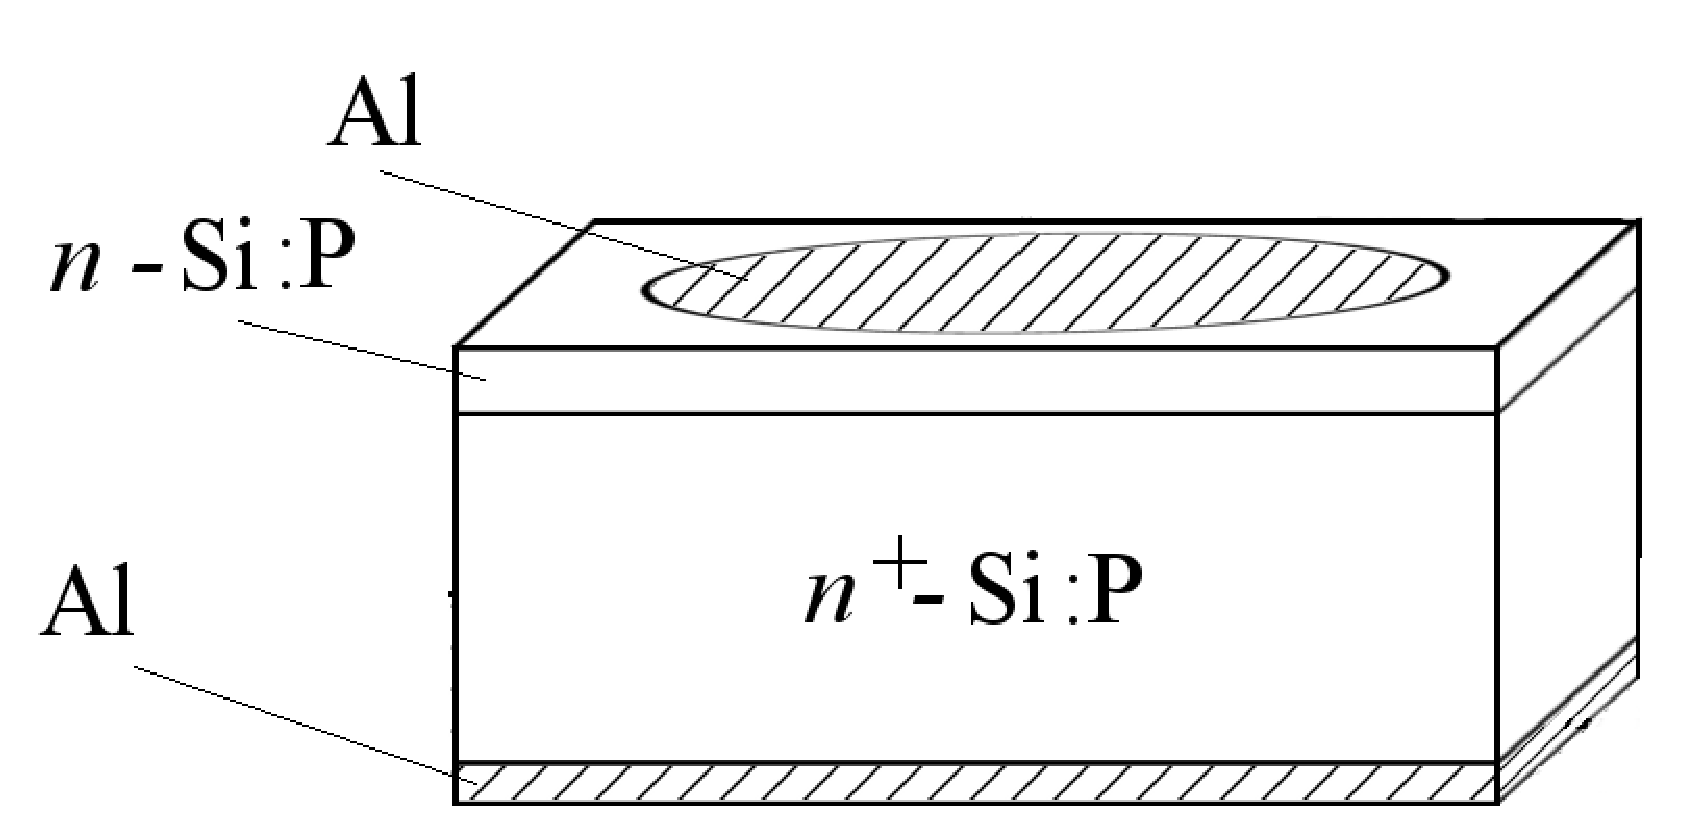
\includegraphics[width=0.65\textwidth]{MSSi}%
\caption{\label{figMSSi}
Структура зразків SSDA.
}
\end{figure}

%Для досліджень використовувалися діоди Шотки з наступною структурою:
%на підкладці $n^+$-Si:Sb (KЭС~0.01, товщина 250~мкм) знаходиться епітаксійний шар $n$-Si:P (товщина 0.2~мкм);
%на поверхні епі-шару створено контакт  Шотки діаметром 2 мм шляхом нанесення шару молібдену;
%на протилежному боці підкладки --- омічний контакт.


В цьому розділі представлені результати дослідження діодів Шотки Al$-n-n^+$--Si---Al,
виготовлених за стандартною технологією \cite{Vorobets:FM2003,StrihaBook1987} на пластинах кремнію КЭФ--1 товщиною $250$~мкм
з орієнтацією (111).
Пластини хімічно очищалися, з неробочої поверхні
повністю видалявся попередньо сформований шар SiO$_2$ для легування фосфором.
На робочій поверхні хімічним травленням створювалися вікна в SiO$_2$ і проводилося очищення
за допомогою іонного пучка.
Потім на робочу поверхню була напилена алюмінієва плівка і проводився процес фотолітографії.
Після цього на протилежну поверхню наносився шар алюмінію товщиною близько 1~мкм і проводився відпал
у інертній атмосфері.
Внаслідок термічної обробки утворювалася структура з випрямляючим контактом на робочій поверхні і омічним на протилежній.

Діаметр контакту Шотки складав 2 мм (площа ДШ $A=3,14\cdot10^{-6}$~м$^2$).
Для контролю рівня легування приповерхневого шару були проведені
вимірювання вольт--фарадних характеристик (ВФХ) досліджуваних структур при кімнатній температурі ($T = 295$~К).
Приклад отриманої залежності наведено на Рис.~\ref{figCV}.
Лінійність залежності $C^{-2}$ від $V$
(де $C$ --- ємність діоду Шотки)
в широкому діапазоні зворотних напруг свідчить про рівномірність легування.
Виявлено, що концентраціями носіїв заряду в епітаксійному шарі $N_d=(1,1\div1,2)\cdot10^{23}$~м$^{-3}$.


\begin{figure}
\center
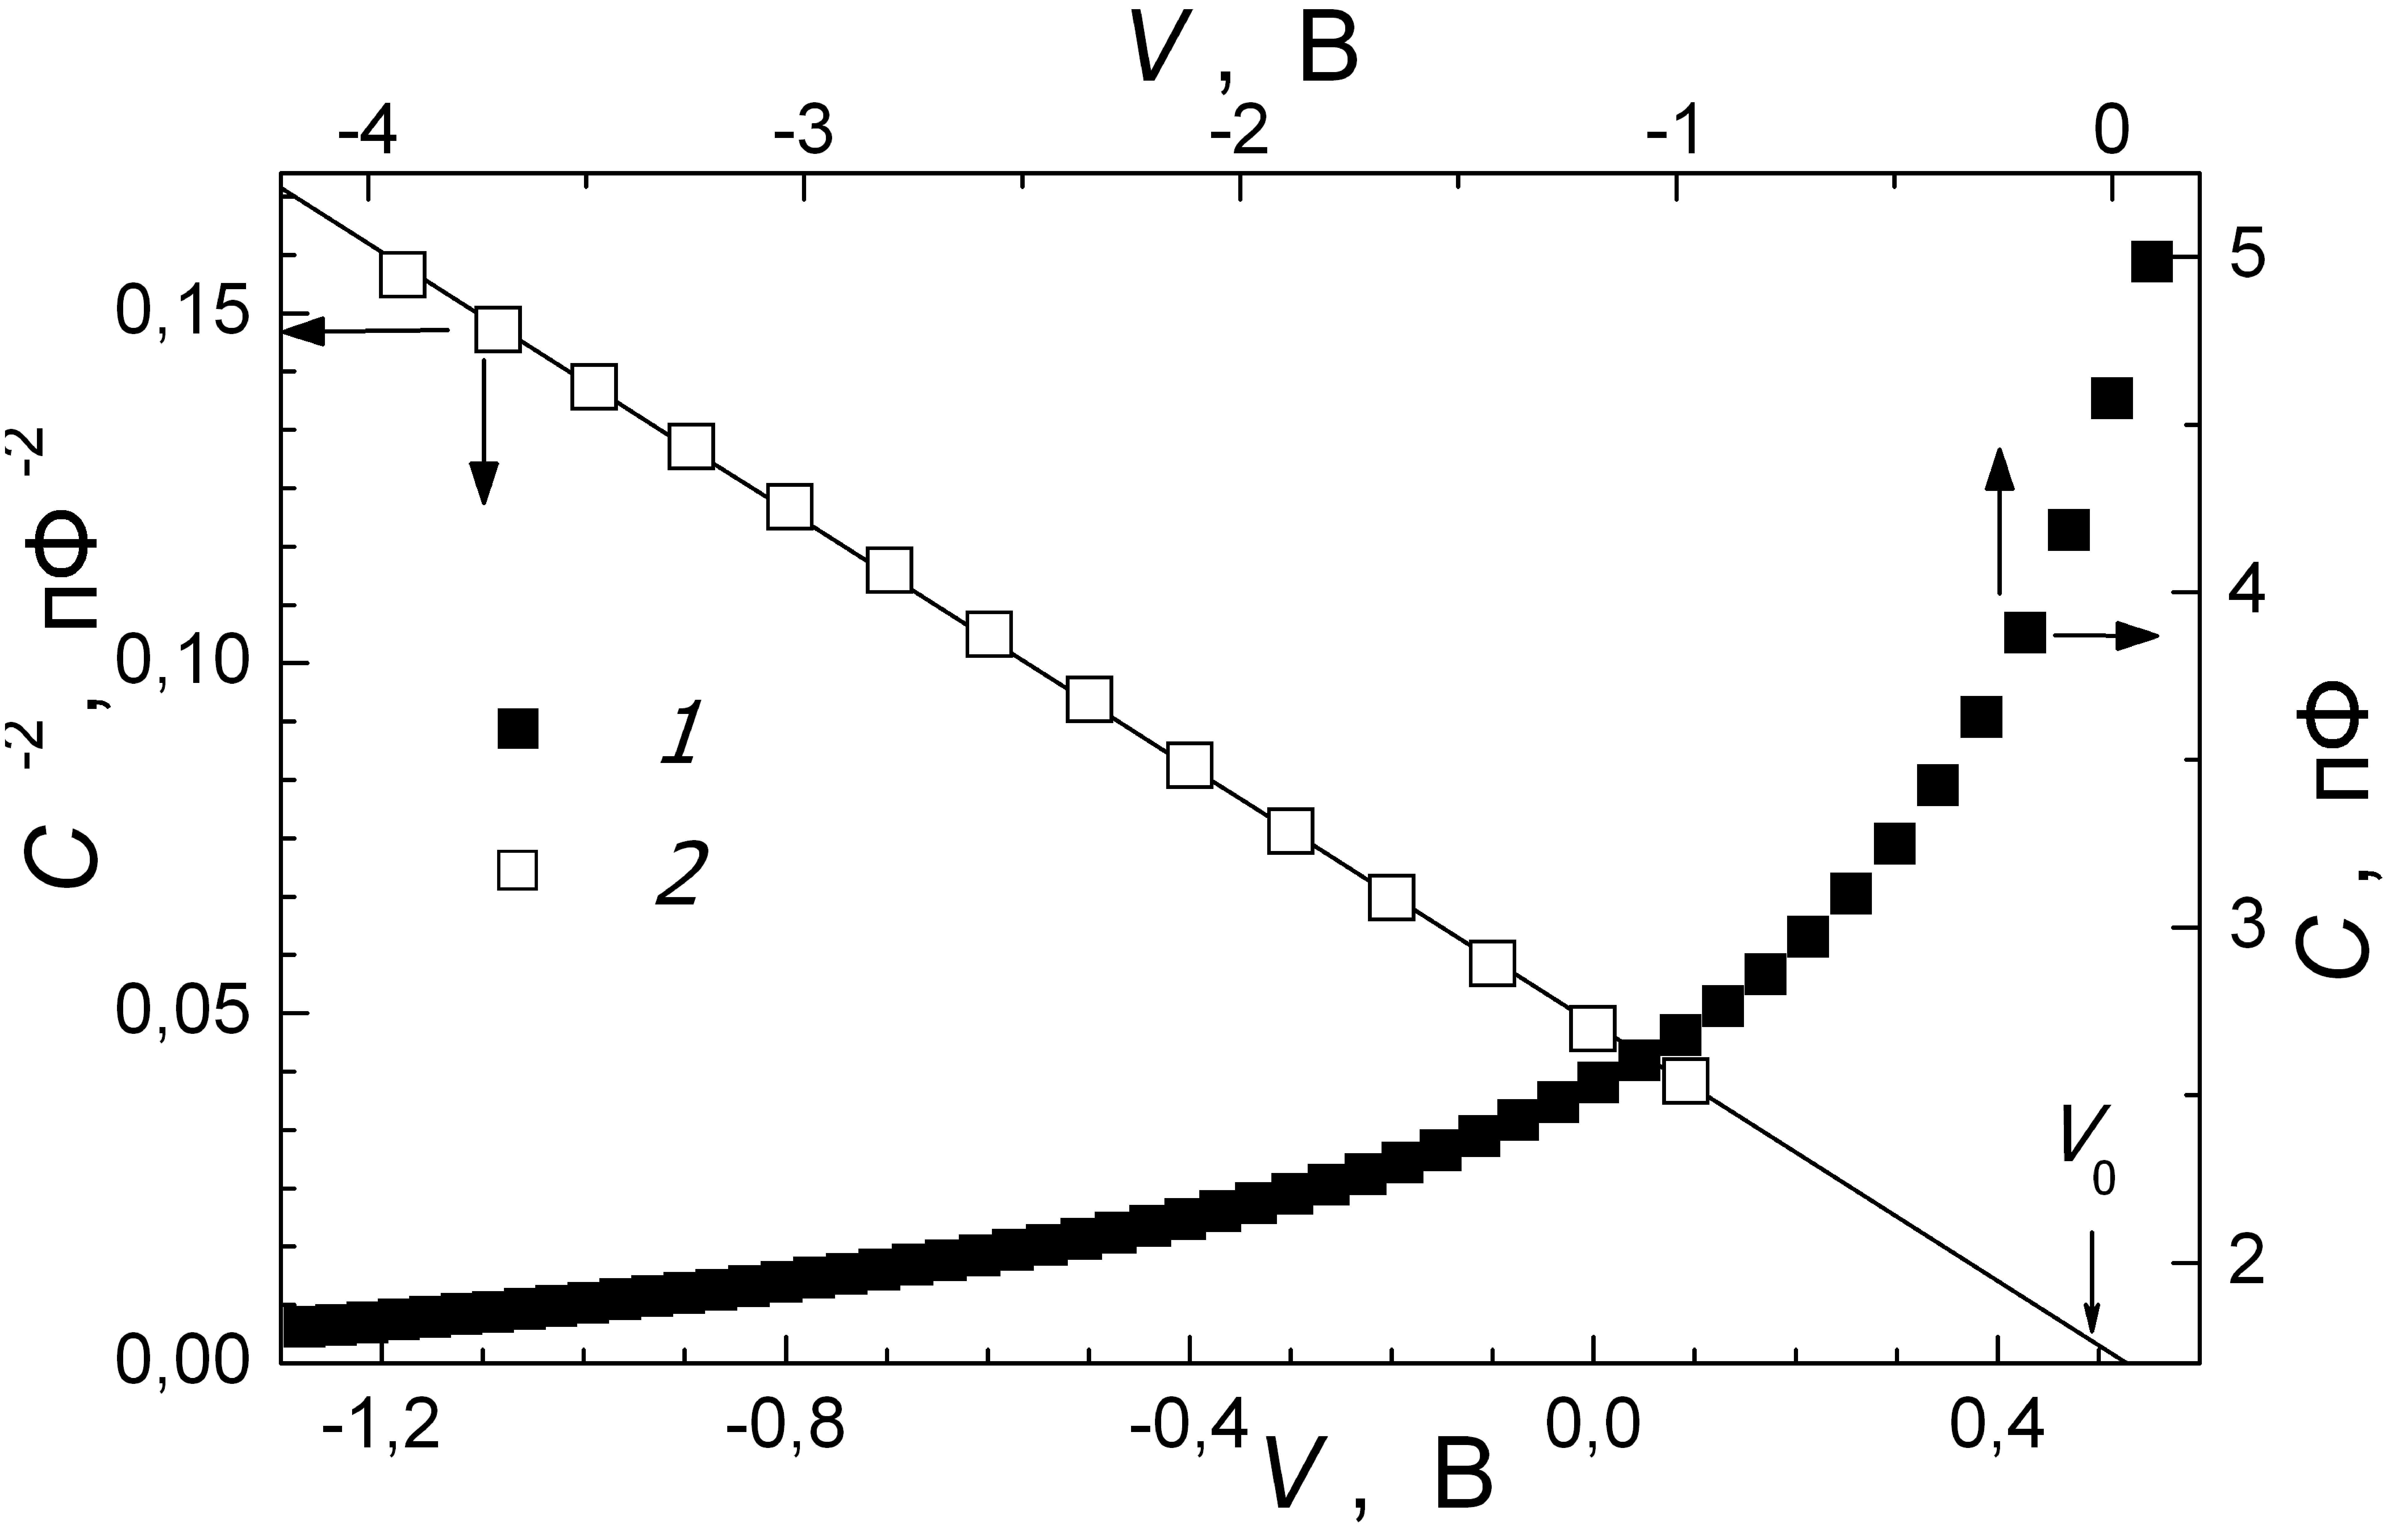
\includegraphics[width=0.7\textwidth]{figCV}
\caption{\label{figCV}
Залежність ємності Al$-n-n^+$--Si---Al діодів Шотки $C$ (крива \emph{1}) та величини $C^{-2}$ (\emph{2}) від прикладеної напруги.
$T=295$~К.
Точки --- експеримент, пряма --- лінійна апроксимація  \emph{2}.
}%
\end{figure}







%В дисертації представлені результати, отримані з використанням кремнієвих ДШ двох типів,
%які ідентичних за структурою, проте відрізняються концентраціями концентраціями носіїв заряду в епітаксійному шарі $N_d$ та
%підкладці $N_s$, а також площею випрямляючого контакту $A$.
%Для контролю рівня легування були виконані вимірювання вольт--фарадних характеристик (ВФХ) досліджуваних структур при кімнатній температурі ($T = 295$~К).
%Параметри структур, а також їх позначення наведені в Таблиці~\ref{tabMSSi}.




Було проведено вимірювання ВАХ даних структур в діапазоні зміни постійного струму $(10^{-9}\div10^{-2})$~А при
прямому та зворотному зміщенні з кроком по напрузі 0.01~В в діапазоні температур $(130\div330)$~К.


\section{Особливості перенесення заряду в структурах Al$-n-n^+$--Si---Al з бар'єром Шотки\label{MSSi_Non}}
\subsection{Перенесення заряду при прямому зміщенні}

%\subsubsection{Особливості аналізу експериментально виміряних ВАХ}

Приклади виміряних прямих ВАХ при різних температурах наведено на рис.~\ref{figIV_SDA}.
Видно, що при температурі більше 250~К прямі ВАХ в напівлогарифмічному масштабі є практично лінійними в інтервалі зміни струму близько трьох порядків.
В той самий час, при $T<210$~K загальний струм можна розділити на дві складові, причому для ВАХ, пов'язаної зі струмом,
який домінує при малих зміщеннях, суттєвим є вплив послідовного опору.
Про це свідчить відхилення від лінійності наведених кривих при при $7\cdot10^{-8}\mbox{A}<I<5\cdot10^{-7}\mbox{A}$.

В літературі \cite{Rhoderick1988,Gromov,Sze2012} показано, що в реальних структурах МН для опису залежності струму від прикладеної прямої напруги
навіть при врахуванні лише термоемісійних процесів замість виразу~(\ref{eqSDIV}) більш доцільно використовувати наступний
\begin{equation}
\label{eqSDIV:2}
I=I_s\exp\left[\frac{q(V-IR_S)}{n_\mathrm{id}kT}\right]\cdot
\left\{1-\exp\left[-\frac{q(V-IR_S)}{kT}\right]\right\}.
\end{equation}
У зв'язку з цим для опису прямих гілок ВАХ було використано вираз
\[
I=I_1+I_2=I_{s1}\exp{\left(\frac{qV}{n_{\mathrm{id},1}kT}\right)}\cdot
\left[1-\exp{\left(-\frac{qV}{kT}\right)}\right]+\]
\begin{equation} \label{eqSDA_IV}
+I_{s2}\exp\left[\frac{q(V-IR_S)}{n_{\mathrm{id},2}kT}\right]\cdot
\left\{1-\exp\left[-\frac{q(V-IR_S)}{kT}\right]\right\},
\end{equation}
де перший доданок $I_1$ є переважаючим при $I>10^{-5}$~A, а другий $I_2$ --- при $I<5\cdot10^{-7}$~A.
Використання двох доданків для опису ВАХ бар'єрних структур широко використовується
в літературі --- див., наприклад, \cite{Arslan,Donoval2010,Huang,GELCZUK2014}.
Зауважимо, що іншим поширеним методом врахування наявності особливостей на ВАХ при малих зміщеннях є введення шунтуючого опору, а не доданку $I_2$.
Проте, на нашу в думку, у даному випадку такий підхід не є виправданим, так як навіть при найменший зміщеннях пряма ділянка ВАХ не є лінійною --- див. вставку на Рис.~\ref{figIV_SDA}.

\begin{figure}
\center
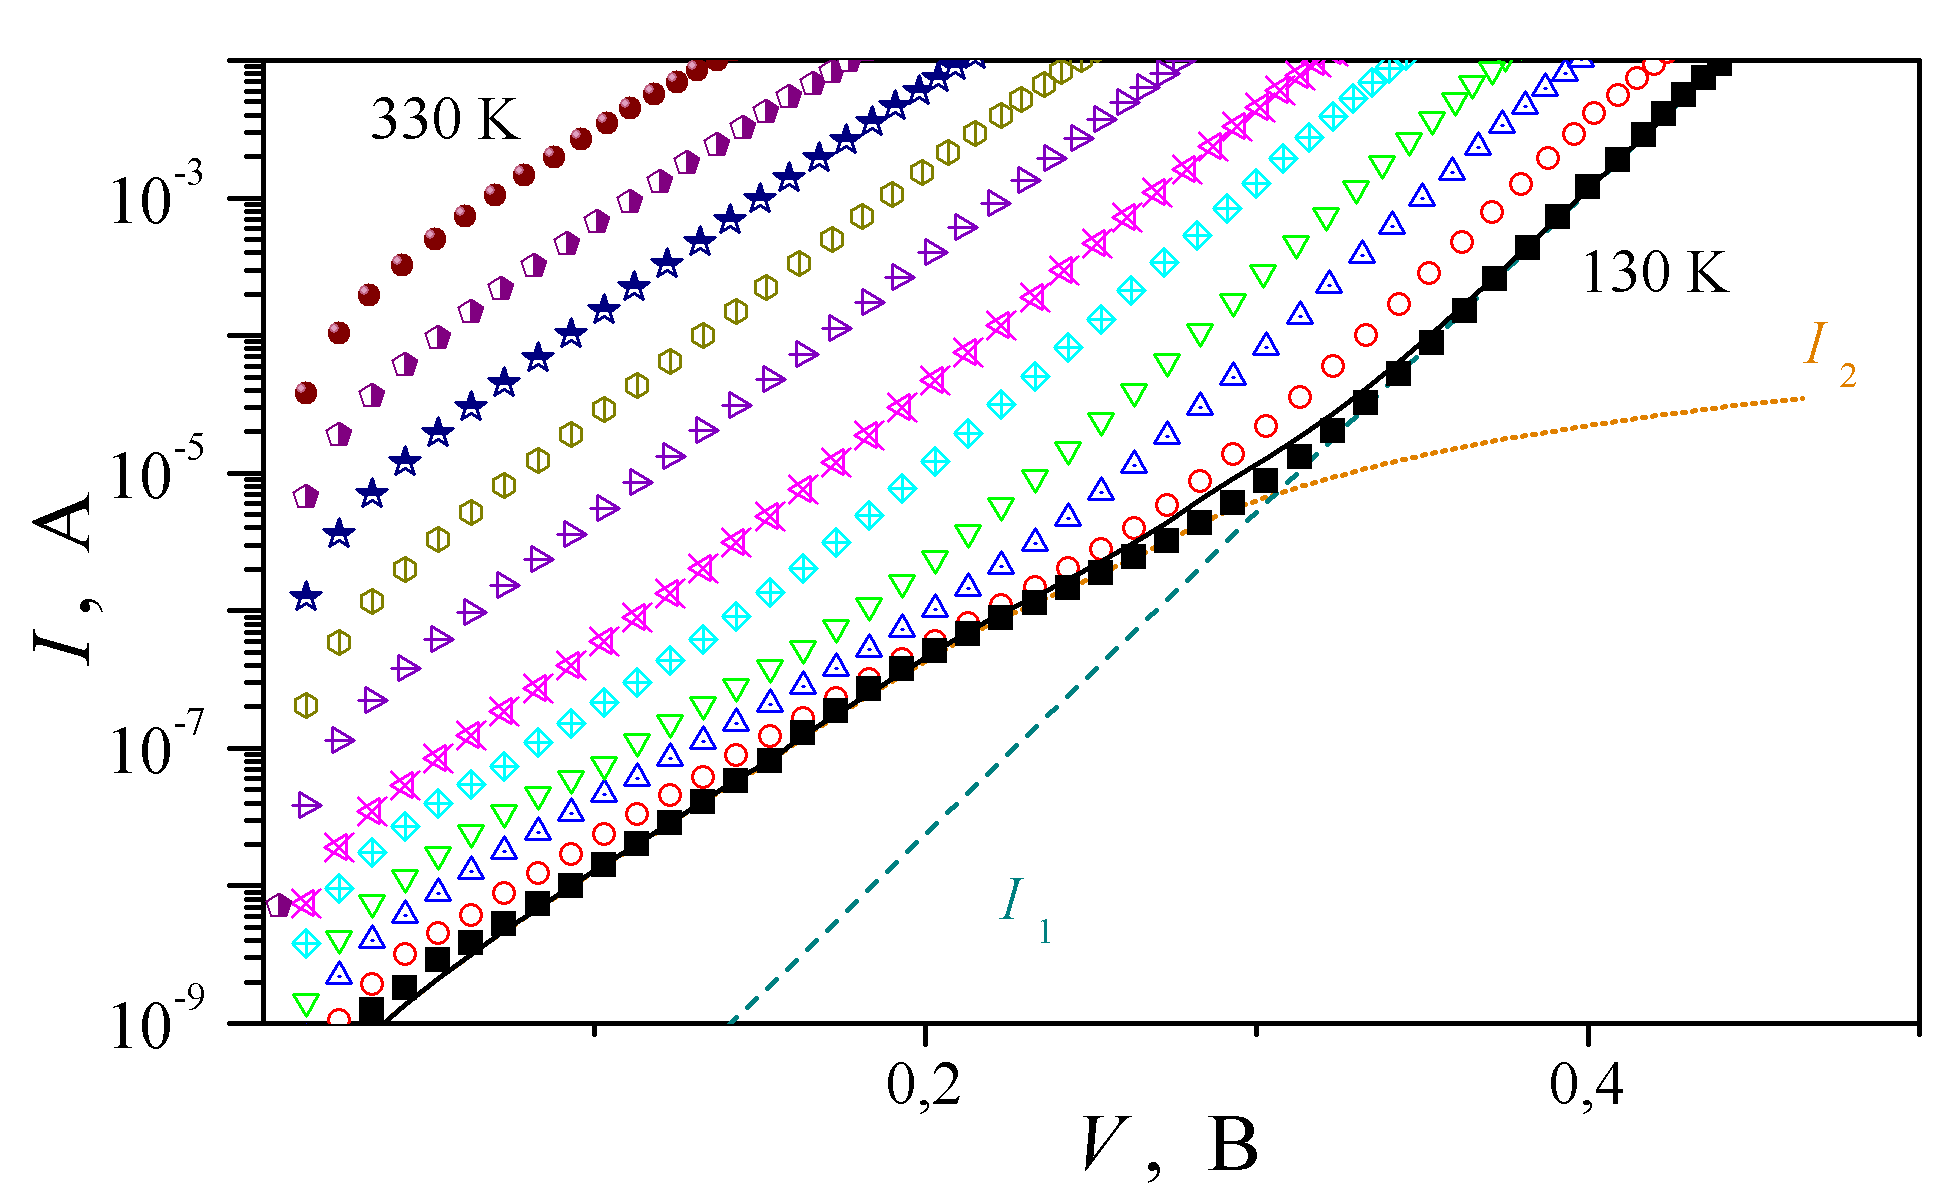
\includegraphics[width=0.8\textwidth]{figIV_SDA}
\caption{\label{figIV_SDA}
Прямі  ділянки ВАХ структур SSDA в температурному діапазоні $130\div330$~К.
Наведено криві, виміряні з кроком 20~К.
Лінії --- апроксимація прямої ВАХ при $T=130$~К за формулою~(\ref{eqSDA_IV}):
штрихова -- струм $I_1$, пунктирна -- $I_2$,
суцільна -- їх сума;
параметри апроксимації $n_{\mathrm{id},1}=1,67$,
$n_{\mathrm{id},2}=2,53$,
$I_{s1}=5,0\cdot10^{-13}$~A,
$I_{s2}=3,8\cdot10^{-10}$~A, $R_{s}=4.1\cdot10^3$~Ом.
На вставці --- початкова ділянка прямої ВАХ при $T=130$~K.
}%
\end{figure}

Для визначення апроксимаційних параметрів використовувалася наступна процедура.
Пряма ВАХ розбивалася на дві ділянки,
для яких $10^{-5}\mbox{A}<I<10^{-2}\mbox{A}$ та
$10^{-9}\mbox{A}<I<10^{-7}\mbox{A}$.
Використовуючи дані першої, виконувалась побудова залежності величини $\ln{{I}/{\left[1-\exp\left(-qV/kT\right)\right]}}$ від $V$, яка надалі
апроксимувалася за методом найменших квадратів прямою,
кутовий коефіцієнт та вільний член якої пов'язані з $n_{\mathrm{id},1}$ та $I_{s1}$ відповідно.
Спираючись на дані другої ділянки ВАХ і використовуючи методи Cheung \cite{Cheung} та Gromov \cite{Gromov}, визначалась величина $R_s$.
Використання двох методів мало на меті підвищити достовірність отриманих даних і воно показало, що отримані обома шляхами значення близькі (в межах 10\%) між собою.
Після визначення $R_s$, будувалась залежність $\ln (I /\{1 - \exp[ -q (V - IR_s) / (kT ) ]\})$ від
ефективної напруги $(V-IR_s)$ і для знаходження $I_{s2}$ та $n_{\mathrm{id},2}$ використовувалася процедура, описана вище.

На рис.~\ref{figIV_SDA} наведено приклад апроксимації експериментальної прямої ВАХ при одній з температур за формулою \eqref{eqSDA_IV} з використанням параметрів,
отриманих за описаною методою.
Видно задовільний збіг розрахованої кривої та експериментальних точок.

У випадку, коли проходження струму через бар'єр визначається ТЕ, то висота бар'єру Шотки при
нульовому зміщенні $\Phi_b$ пов'язана зі струмом насичення співвідношенням \cite{Rhoderick1988}:
\begin{equation}
\label{eqFb:TE}
\Phi_b=\left(\frac{kT}{q}\right)\cdot\ln\left(\frac{AA^*T^2}{I_s}\right).
\end{equation}
Отримані температурні залежності для висот бар'єрів та факторів неідеальності обох компонент струму наведено на Рис.~\ref{figFbT_SDA}.

%Розглянемо спочатку особливості струму, переважаючого при високих температурах та великих зміщеннях ($I_1$).


\begin{figure}
\center
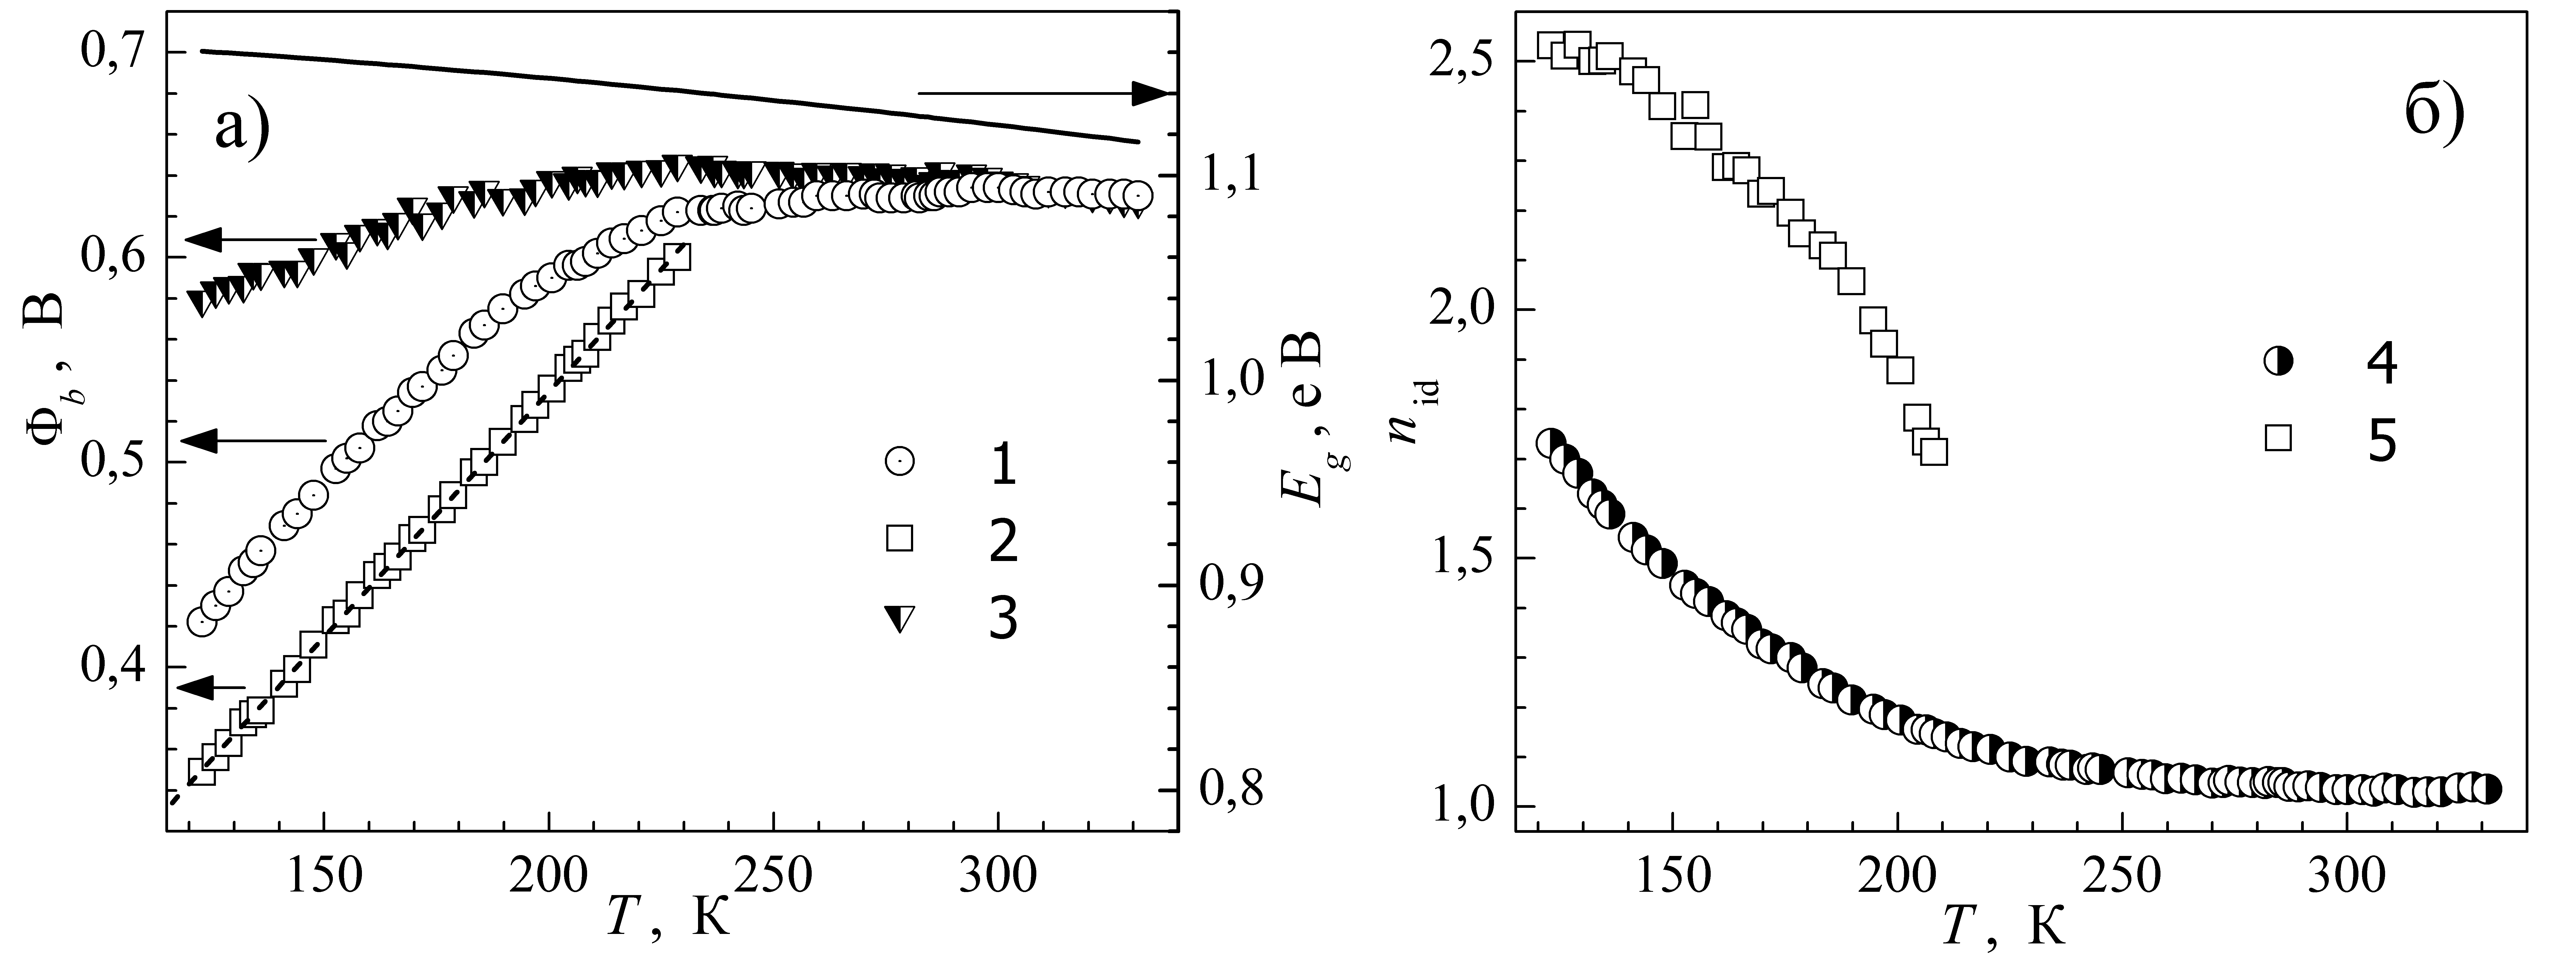
\includegraphics[width=0.5\textwidth]{figFbT_SDA}
\caption{\label{figFbT_SDA}
Температурні залежності висоти бар'єру (а) та фактору неідеальності (б) структури SSDA.
1 -- $\Phi_{b1}$,
2 -- $\Phi_{b2}$,
3 -- $\Phi_{b1}^\mathrm{eff}$ ,
4 -- $n_{\mathrm{id},1}$, 5 -- $n_{\mathrm{id},2}$.
Пунктир -- лінійна апроксимація кривої 2.
Також приведено температурну залежність ширини забороненої зони Si (а, суцільна лінія).
}%
\end{figure}

З рисунка видно, що при збільшенні температури фактор неідеальності зменшується, наближаючись
до одиниці при кімнатних температурах.
Як відомо, що температурна залежність фактору неідеальності залежить від механізму перенесення заряду.
Зокрема, для ідеального випадку ТЕ очікується, що $n_{\mathrm{id}}=1$ при будь--яких температурах.
Проте для реальних контактів така рівність не спостерігається і для опису залежності $n_{\mathrm{id}}(T)$
часто використовують вираз \cite{Rhoderick1988, Sze2012}
\begin{equation}\label{eqN_T:TE}
n_{\mathrm{id}}=1+\frac{T_0}{T},
\end{equation}
де $T_0$ --- певна константа, що не залежить від температури та зміщення в широкому температурному інтервалі.

Проте залежність, подібна до зображеної на Рис.~\ref{figFbT_SDA},б очікується
і у випадку, коли домінуючим механізмом є термопольова  емісія (ТПЕ), польова емісія або тунелювання за участю глибоких рівнів
\cite{Rhoderick1988,Evstropov,Soylu,JYOTHI2015,OZAVCI2013,Abhishek}.
В цьому випадку
\begin{equation}\label{eqN_T:TFE}
n_{\mathrm{id}}^\mathrm{T}=\frac{E_{00}}{kT}\cdot\coth\left(\frac{E_{00}}{kT}\right),
\end{equation}
де $E_{00}$ --- характеристична енергія тунелювання.


\begin{figure}
\center
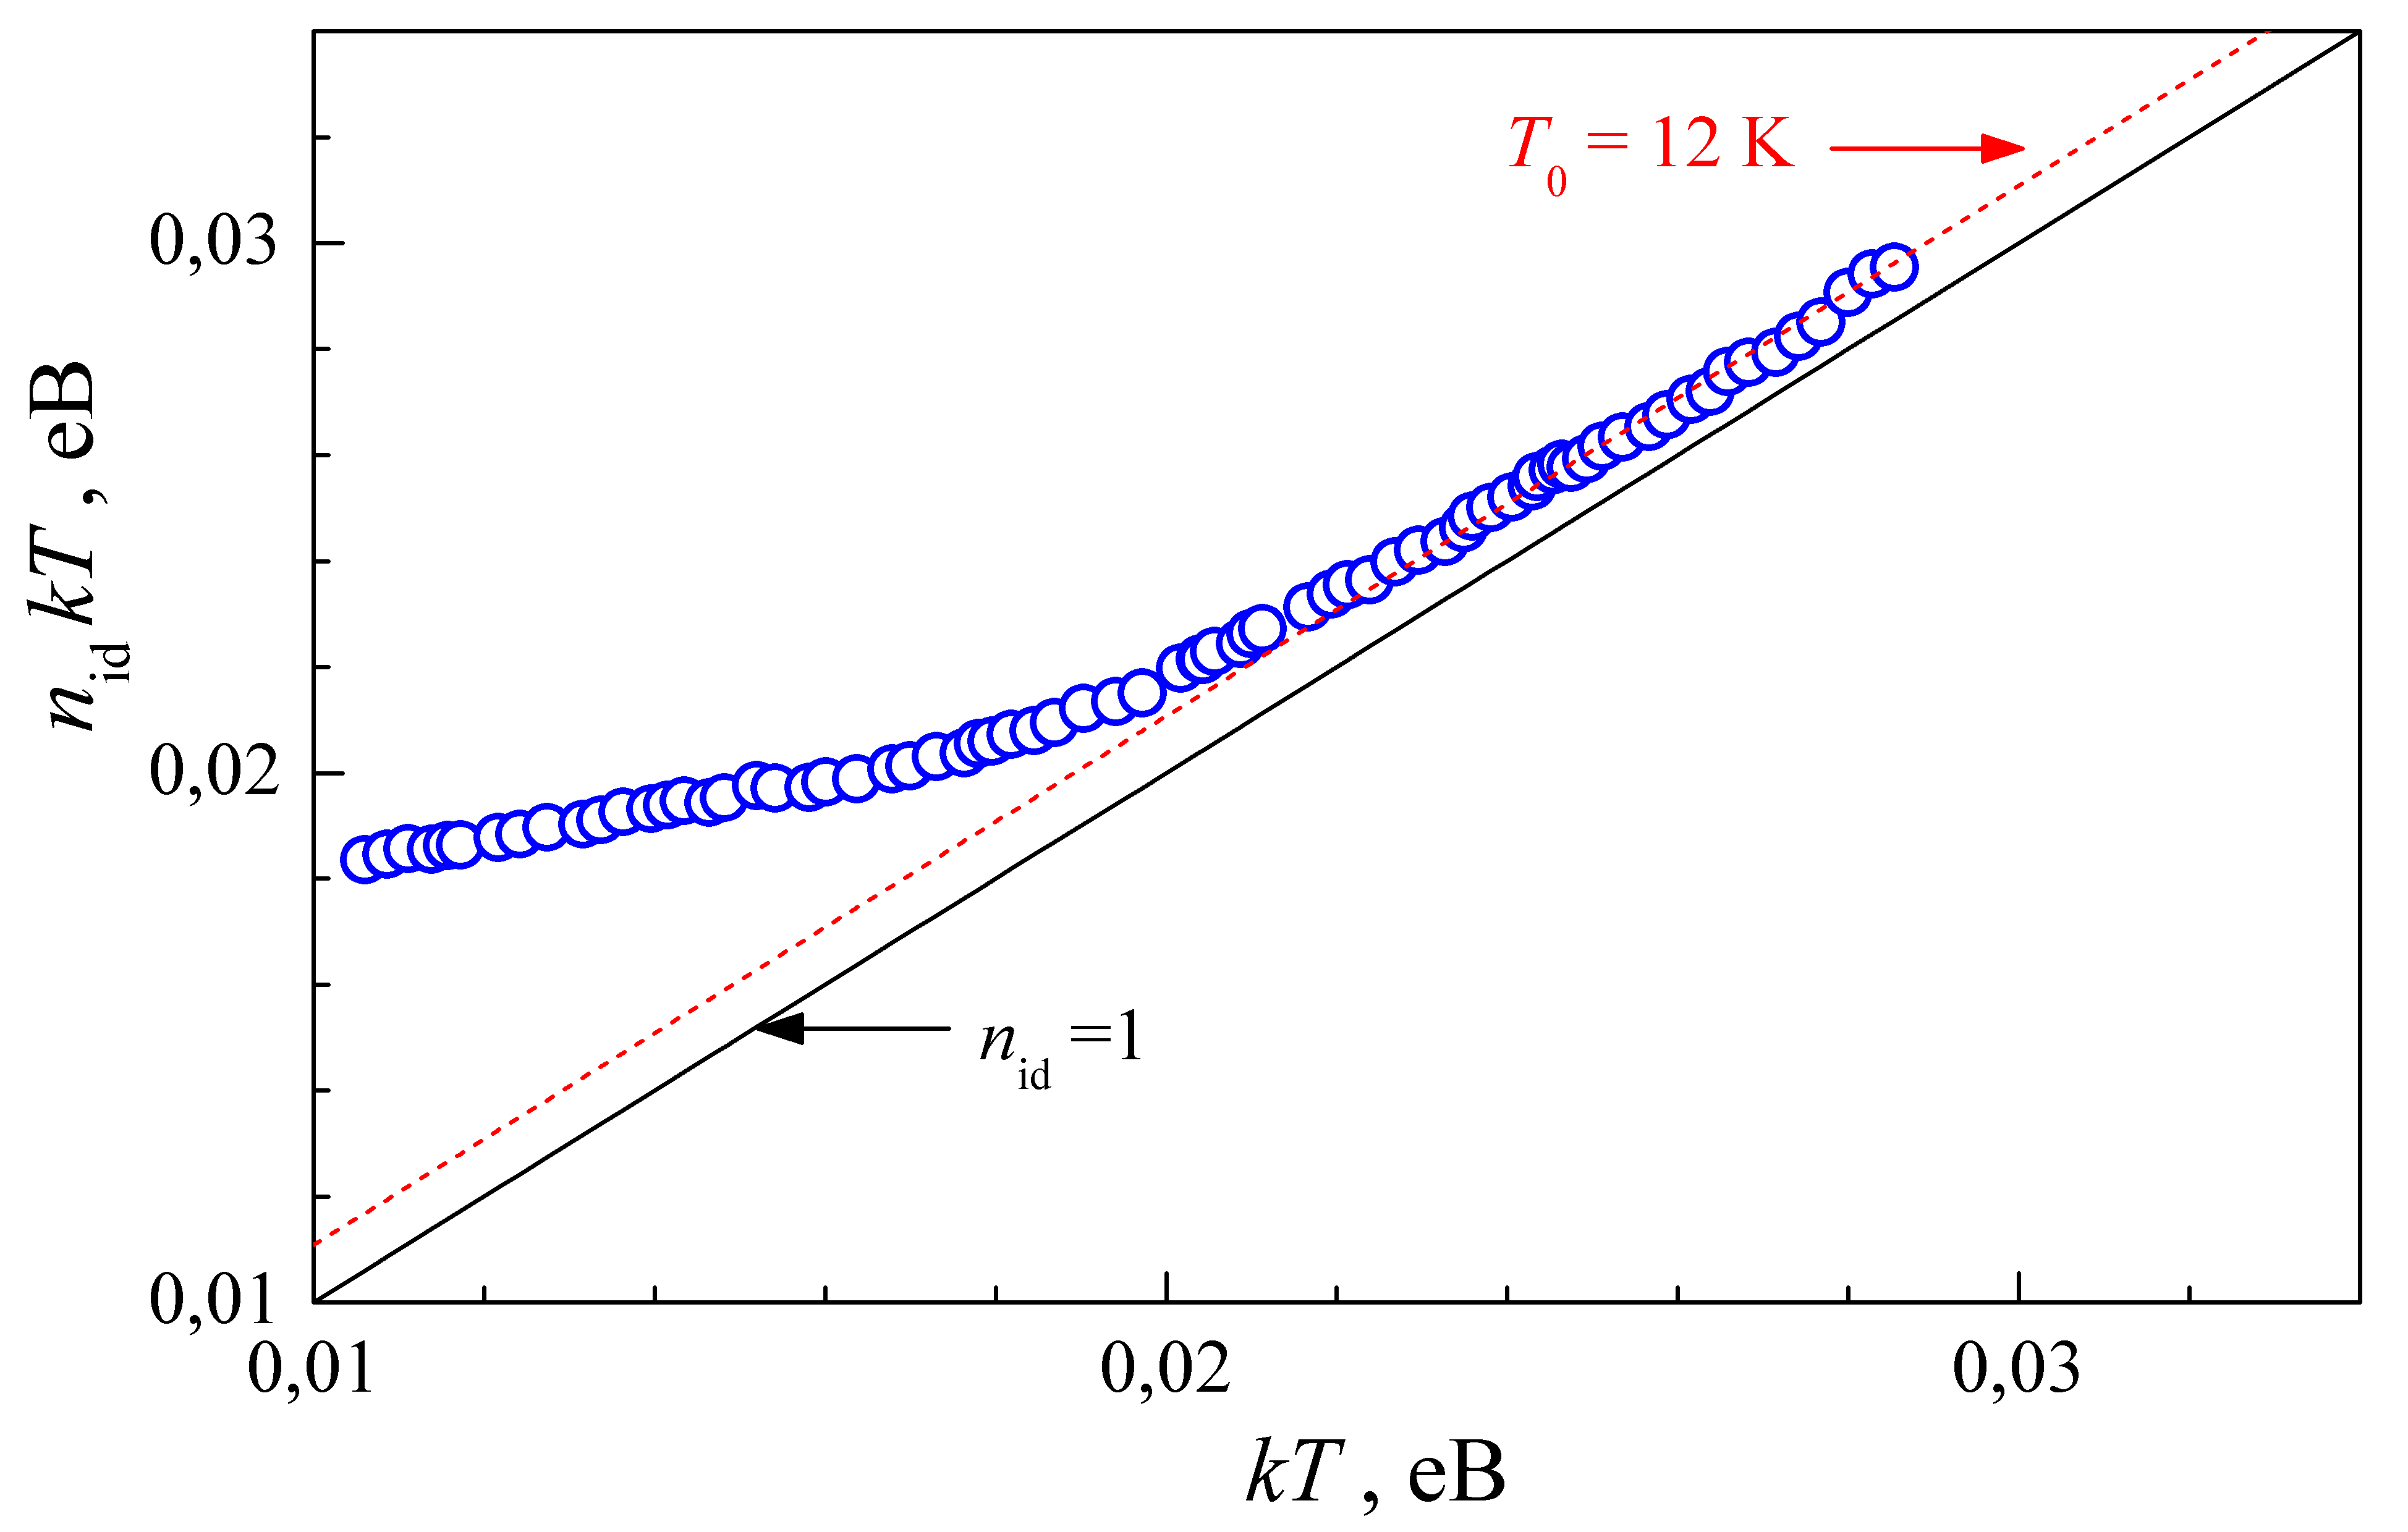
\includegraphics[width=0.75\textwidth]{figNT_SDA}
\caption{\label{figNT_SDA}
Температурна залежність оберненого нахилу ВАХ.
1 --- $n_{\mathrm{id},1}$;
2 --- $n_{\mathrm{id},2}$.
Пунктир --- теоретичні криві відповідно до формул (\ref{eqN_T:TE}) (криві А та В)
та (\ref{eqN_T:TFE}) (криві С-G).
$T_0$, K: 12 (A), 206 (B).
$E_{00}$, мВ: 12 (С), 17 (D), 22 (E), 27 (F), 32 (G).
Також наведено ідеальний випадок ($n_{\mathrm{id}}=1$) --- пряма суцільна лінія.
}%
\end{figure}

На Рис.~\ref{figNT_SDA} наведено експериментально отримані залежності факторів неідеальності від оберненої температури
для обох струмових компонент та декілька кривих, розрахованих з використанням виразів (\ref{eqN_T:TE}) та (\ref{eqN_T:TFE}).
Видно, що отримані дані для $n_{\mathrm{id},1}$ (при $T>220$~K) та $n_{\mathrm{id},2}$ задовільно описуються
виразом (\ref{eqN_T:TE}) при $T_0=12$~К та $T_0=206$~К, відповідно,
що свідчить на користь ТЕ як основного механізму перенесення заряду.
Зауважимо, що при ТПЕ
\begin{equation}\label{eqE00:TFE}
E_{00}=\frac{\hbar}{2}\sqrt{\frac{N_d}{m^*\varepsilon_s\varepsilon_0}},
\end{equation}
($m^*$ -- ефективна маса електрону, $m^*=1.08\cdot9.11\cdot10^{-31}$~кг)
і тому для досліджених зразків та температурного діапазону очікувалось, що при домінуванні цього механізму $n\approx1$.



Раніше вже згадувалося, для однорідного контакту Шотки теоретично \cite{Rhoderick1988} та експериментально \cite{Aboelfotoh,Zhua} показано,
що при підвищенні температури за умови домінування термоелектронної емісії ВБШ має зменшуватися,
причому температурні коефіцієнти змін $\Phi_b$ та  $E_g$ дуже близькі між собою.
На Рис.~\ref{figFbT_SDA},а також наведена температурна залежність $E_g$, розрахована з використанням
виразу (\ref{eqEg}).
Для дослідженої структури спостерігається зворотна тенденція: ВБШ зі збільшенням температури зростає практично у всьому
діапазоні
і лише для компоненти $I_1$ поблизу кімнатної температури поведінка $\Phi_b$ нагадує $E_g$.

З іншого боку, відомо, що ВБШ, визначена за допомогою ВАХ, може відрізнятися від реальної.
Зокрема, в роботі \cite{Bozhkov} стверджується про необхідність проведення вимірів при сталому струмі через контакт
і пропонується для оцінки ефективної висоти бар'єру $\Phi_{b}^\mathrm{eff}$ використовувати вираз
\begin{equation}\label{eqBoz}
\Phi_{b}^\mathrm{eff}=n_{Ic}\Phi_b-(n_{Ic}-1)\cdot\frac{kT}{q}\cdot\ln\left(\frac{AA^*T^2}{I_c}\right),
\end{equation}
де
$n_{Ic}$ --- фактор неідеальності при певному сталому значенні струму $I_c$.
В роботі \cite{Bozhkov} також показано, що у випадку ТЕ через однорідний контакт $\Phi_{b}^\mathrm{eff}$ майже збігається за величиною
з реальною висотою бар'єру і має з нею однакову температурну залежність.

Результати обчислення $\Phi_{b1}^\mathrm{eff}$ для $I_{s1}$ згідно з формулою (\ref{eqBoz}) при $I_c=10^{-3}$~А показані на Рис.~\ref{figFbT_SDA}, крива 3.
Видно, що хоча величина $\Phi_{b1}^\mathrm{eff}$ і змінюється в значно меншому діапазоні,
проте її температурна залежність також відрізняється від поведінки $E_g$, особливо при низьких температурах.


Якщо ТЕ є домінуючим механізмом перенесення заряду, то параметр $A^*$ може бути
визначений \cite{Rhoderick1988,Schroder2006} шляхом побудови так званої залежності Річардсона,
тобто залежності величини $\ln(I_s/T^2)$ від $(kT)^{-1}$.
Згідно з (\ref{eqFb:TE}), вона має описуватися виразом
\begin{equation}\label{eqRich}
\ln\left(\frac{I_s}{T^2}\right)=\ln(AA^*)-\frac{q\Phi_b}{kT},
\end{equation}
тобто залежність Річардсона має бути прямою, нахил якої визначається ВБШ,
я точка перетину з вертикальною віссю --- константою $A^*$.


Відповідна залежність, побудована для даних, отриманих для складової $I_1$ наведена
на Рис.~\ref{figRich_SDA}, крива 1.
Видно, що лінійна залежність дійсно спостерігається, але не у всьому діапазоні температур, а у двох окремих піддіапазонах.
Шляхом апроксимації в діапазоні $(130\div220)$~К були отримані значення $3,7\cdot10^{-10}$~А$\cdot$см$^{-2}\cdot$К$^{-2}$ та
$0,141$~В для сталої Річардсона та висоти бар'єру, відповідно,
тоді як для діапазону $(230\div330)$~К ---
$30$~А$\cdot$см$^{-2}\cdot$К$^{-2}$ та $0,599$~В.
Величини також наведені в Таблиці~\ref{tabPar:SSDA}.
Очевидно, що отримані значення сталої Річардсона суттєво відрізняються від літературних даних
для кремнію (112~А$\cdot$см$^{-2}\cdot$К$^{-2}$).


\begin{figure}
\center
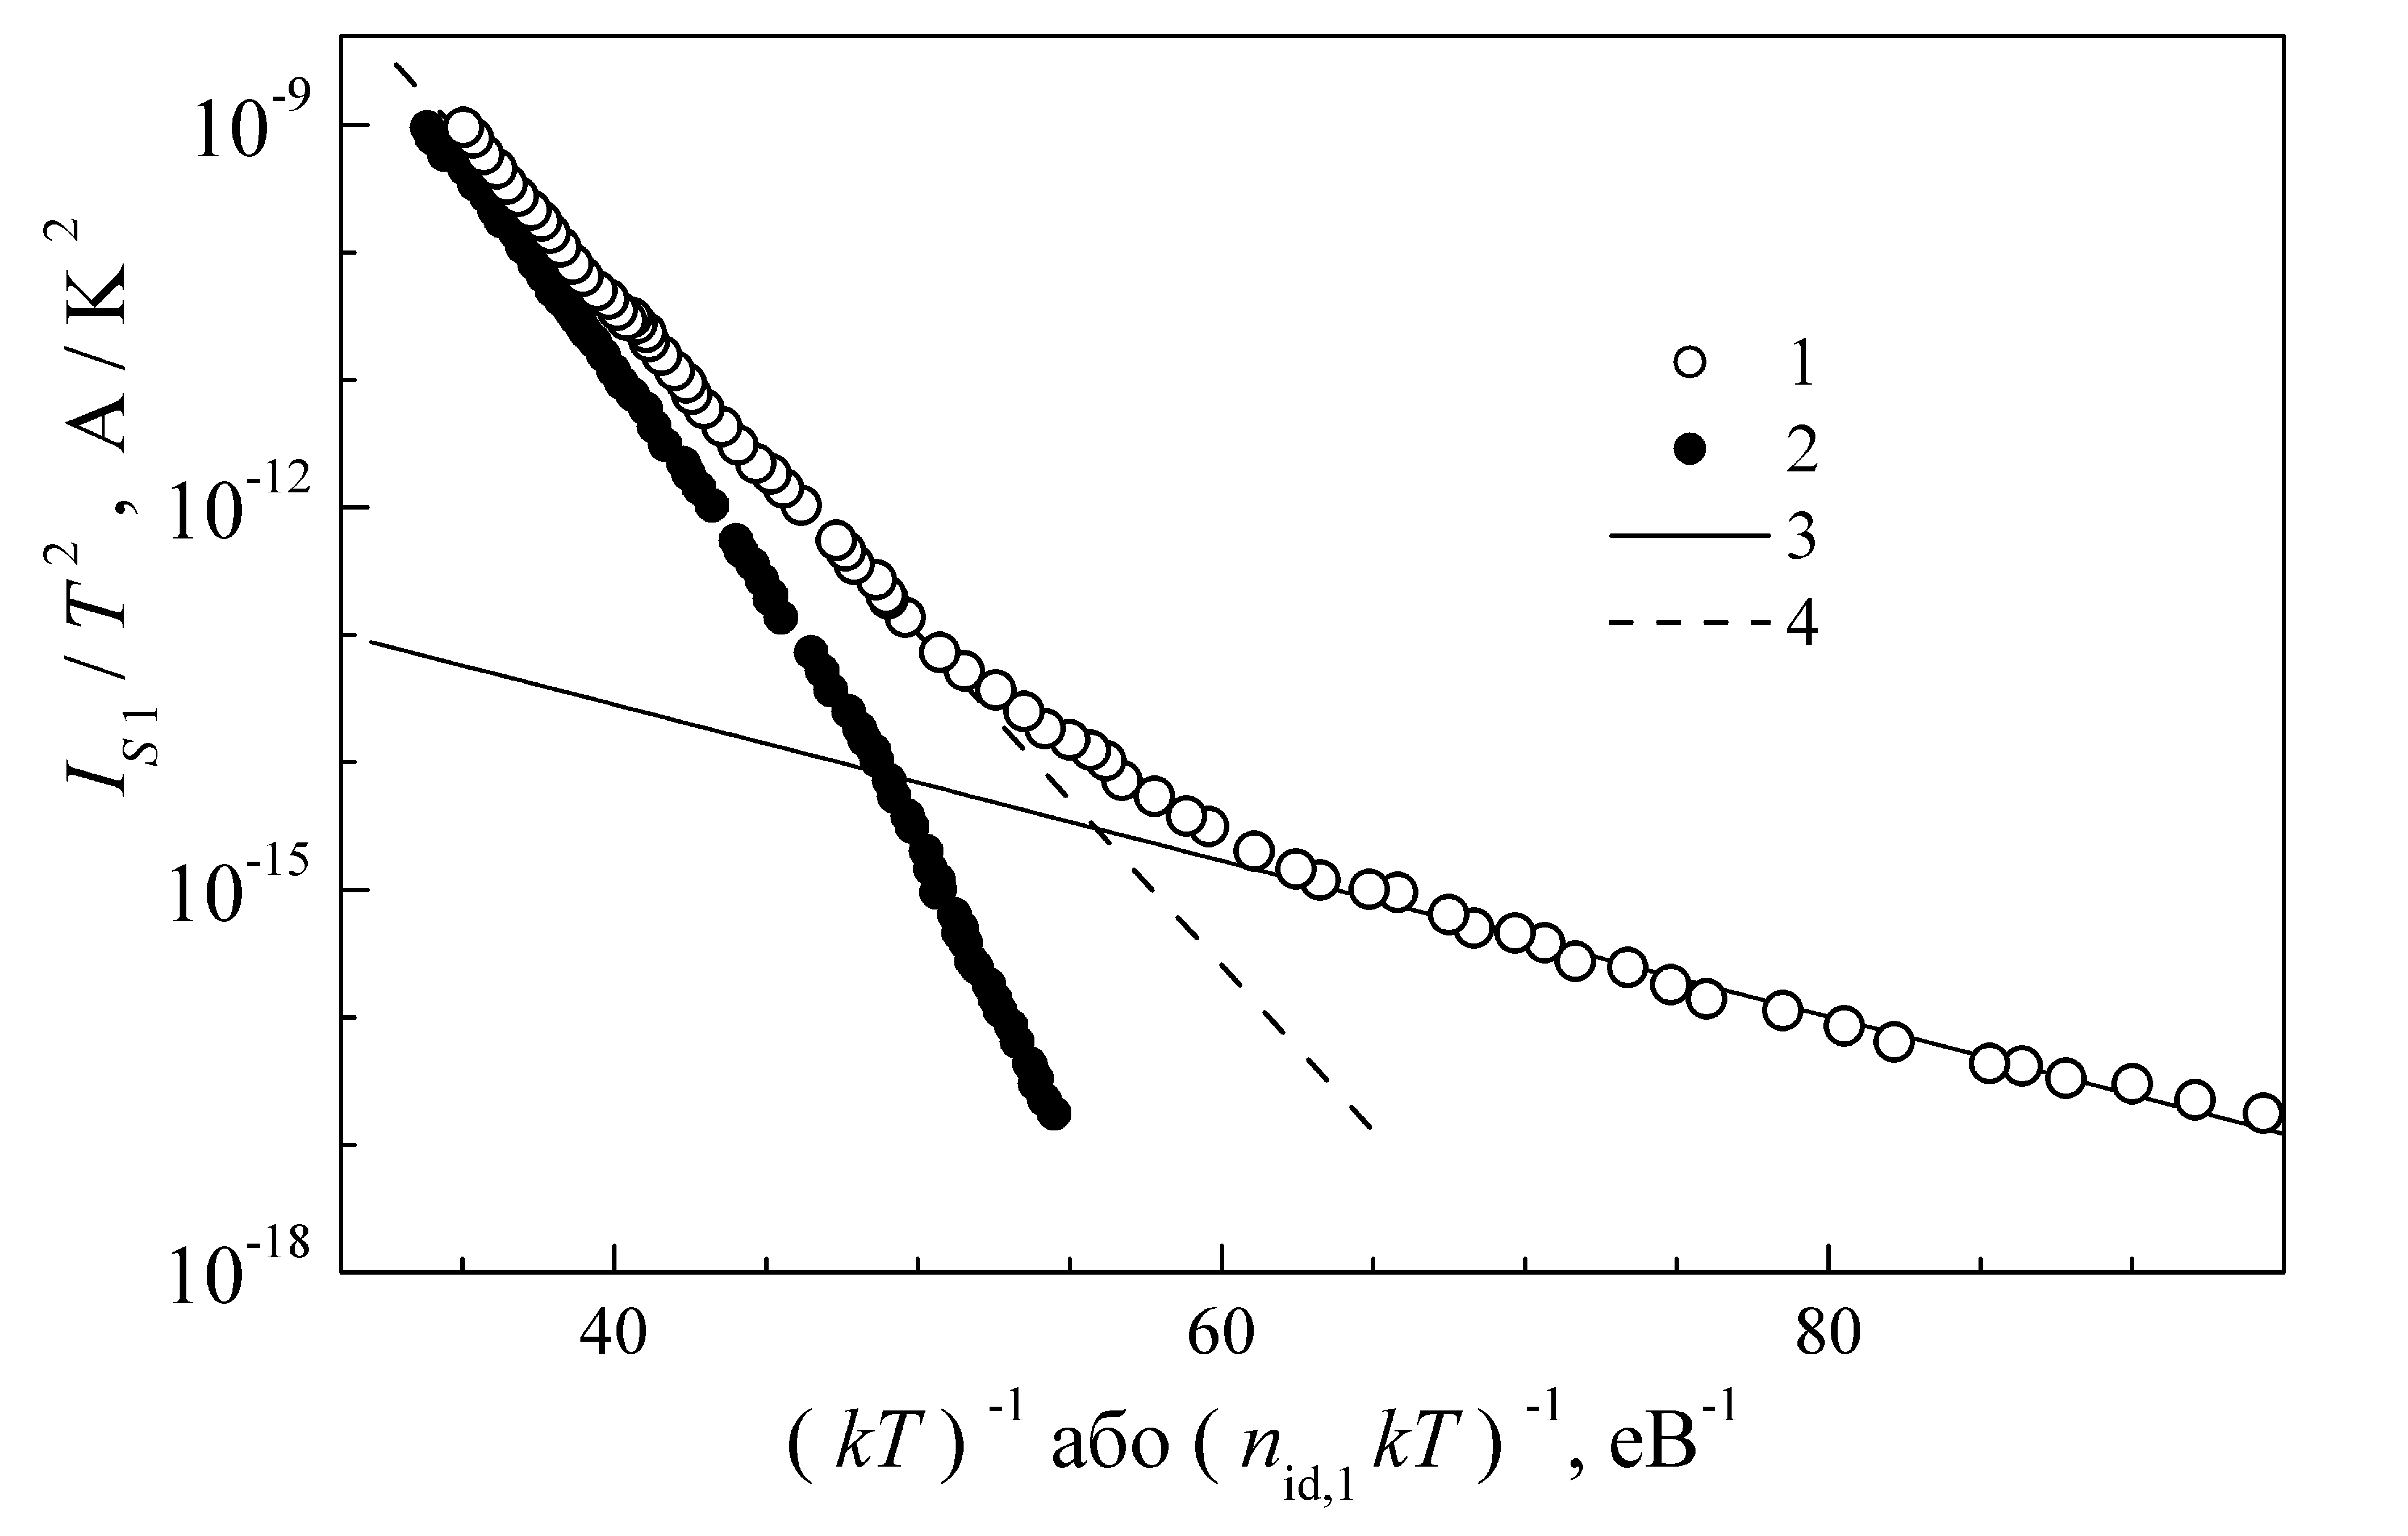
\includegraphics[width=0.7\textwidth]{figRich_SDA}
\caption{\label{figRich_SDA}
Залежності Річардсона, побудовані для високотемпературної компоненти струму $I_1$
за формулами (\ref{eqRich}) (крива 1) та (\ref{eqRichB}) (крива 2).
Прямі --- лінійна апроксимація даних кривої 1 в діапазонах $T=(130\div220)$~К (3, суцільна)
та $T=(230\div330)$~К (4, пунктир).
}%
\end{figure}



\begin{table}
\caption{\label{tabPar:SSDA}Параметри, визначені для високотемпературної складової струму неопромінених структур SSDA.
}
\center
\begin{tabular}{|l|c|c|}
\hline
\multicolumn{1}{|c|}{Параметр:}& \multicolumn{2}{c|}{Температурний інтервал}\\ \cline{2-3}
метод визначення&$130\div220$~K&$230\div330$~K\\
\hline
%$A^*_R$, А$\cdot$см$^{-2}\cdot$К$^{-2}$&$3.7\cdot10^{-10}$&32\\ \hline
\multicolumn{1}{|c|}{$A^*$, А$\cdot$см$^{-2}\cdot$К$^{-2}$:}&&\\
залежність Річардсона (\ref{eqRich})&$(3,7\pm0,8)\cdot10^{-10}$&$32\pm10$\\
видозмінена залежність Річардсона (\ref{eqRichB})&$(3,0\pm0,6)\cdot10^{8}$&$40\pm8$\\
видозмінена залежність Річардсона (\ref{eqRich:Mod})&$122\pm20$&$112\pm8$\\
література  \cite{Schroder2006}& \multicolumn{2}{c|}{$\,\,\,\,\,\,\,\,\,\,\,\,$   112}\\ \hline
\multicolumn{1}{|c|}{$\Phi_b$, мВ:}&&\\
залежність Річардсона (\ref{eqRich})&141$\pm$4&599$\pm$3\\
видозмінена залежність Річардсона (\ref{eqRichB})&1090$\pm$10&751$\pm$5\\
залежність $\Phi_b=f(\frac{1}{2kT})$&872$\pm$4&663$\pm$3\\
залежність $\Phi_b=f(n_\mathrm{id})$&646$\pm$5&640$\pm$20\\
видозмінена залежність Річардсона (\ref{eqRich:Mod})&872$\pm$3&662$\pm$3\\
ВФХ &&689$\pm$2\\
\hline
залежність $\Phi_b=f(\frac{1}{2kT})$:&&\\
\multicolumn{1}{|c|}{$\sigma_{\Phi0}$, мВ} &99$\pm$1&40$\pm$5\\
\multicolumn{1}{|c|}{$\rho_2$, $10^{-2}$} &33$\pm$1&12$\pm$1\\
\multicolumn{1}{|c|}{$\rho_3$, мВ }&17,0$\pm$0,3&8,0$\pm$0,3\\
\hline
\end{tabular}
\end{table}



У роботі \cite{Aldemir} показано, що
У випадку суттєвого відхилення від ідеальності (величина $n_\mathrm{id}$ значно більша за одиницю)
для визначення $A^*$ можна також використовувати \cite{Aldemir,Mohan} видозмінену залежність Річардсона,
відкладаючи по осі абсцис не $(kT)^{-1}$, а $(n_\mathrm{id} kT)^{-1}$:
\begin{equation}\label{eqRichB}
\ln\left(\frac{I_s}{T^2}\right)=\ln(AA^*)-\frac{q\Phi_b}{n_\mathrm{id}kT},
\end{equation}
Проте для нашого випадку і видозмінена залежність Річардсона (Рис.~\ref{figRich_SDA}, крива 2) не є лінійною для всього
температурного діапазону, а отримані значення $A^*$ (див. Таблицю~\ref{tabPar:SSDA}) суттєво відрізняються
від табличних.

Узагальнюючи вищенаведене, необхідно визнати, що отримані результати неможливо пояснити з точки зору теорії ТЕ через однорідний контакт.


З іншого боку, відмінності між експериментально виявленою температурною залежністю ВБШ та очікуваною теоретично нерідко
пов'язують із неоднорідністю границі розділу між металом та напівпровідником \cite{Dokme}.
Впливу неоднорідності можна позбутися розглядаючи ВБШ за умови плоских зон (<<flat band condition>>) $\Phi_{b}^\mathrm{FB}$:
\begin{equation}
\label{eqFbfb}
\Phi_{b}^\mathrm{FB}=n_\mathrm{id}\Phi_{b}-(n_\mathrm{id}-1)V_n\,,
\end{equation}
де
\begin{equation}
\label{eqVn}
qV_n=kT\ln\left(\frac{N_c}{N_d}\right)
\end{equation}
різниця енергій між дном зони провідності та положенням рівня Фермі в об'ємі напівпровідника,
так званий <<bulk potential>>.
На Рис.~\ref{figFbfb_SDA} наведена температурна залежність $\Phi_{b}^\mathrm{FB}$, розрахована для високотемпературної компоненти $I_1$.
Зауважимо, що на рисунку також наведена температурна залежність ширини забороненої зони, причому
масштаби осей $\Phi_{b}^\mathrm{FB}$ та $E_g$ однакові.
З рисунка видно, що поведінка ВБШ в наближенні плоских зон та ширини забороненої зони дуже подібні,
що свідчить про те, що механізмом перенесення заряду в досліджуваних структурах може бути ТЕ через неоднорідний бар'єр.


\begin{figure}
\center

\includegraphics[width=0.7\textwidth]{figFbfb_SDA}
\caption{\label{figFbfb_SDA}
Температурні залежності ВБШ в наближені плоских зон (точки, права вісь), розрахованої
для високотемпературної компоненти струму $I_1$, та ширина забороненої зони (пунктир, ліва вісь).
}%
\end{figure}

В літературі для пояснення експериментально отриманих ВАХ структур МН використовуються два
підходи \cite{Sarpatwari, Tascioglu2010, Yildirim2010, Mamor, Iucolano2007JAP, Iucolano2007APL}, які дозволяють
%\cite{Sarpatwari, Aydemir, Turut, Mamor, Iucolano, Iucolano2}.
врахувати неоднорідність бар'ру Шотки,
схематично ілюстровані за допомогою Рис.~\ref{figFbModel}.
Згідно з першим підходом, запропонованим в \cite{Werner}, вважається, що контакт між металом та напівпровідником
змінюються від точки до точки (Рис.~\ref{figFbModel},а),  просторовий розподіл ВБШ  може бути описаний розподілом Гауса:
\begin{equation}\label{eqFbWerner}
  P(\Phi_{b}^j)=\frac{1}{\sigma_\Phi\sqrt{2\pi}}\exp\left[-\frac{(\Phi_{b}^j-\overline{\Phi}_{b})^2}{2\sigma_\Phi^2}\right]\,,
\end{equation}
де
$P(\Phi_{b}^j)$ --- ймовірність того, що значення висоти бар'єру в певній точці дорівнює $\Phi_{b}^j$,
$\overline{\Phi}_{b}$ --- середнє значення ВБШ,
$\sigma_\Phi$ --- стандартне відхилення висоти бар'єру, показник однорідності контакту.
Також вважається, що $\overline{\Phi}_{b}$ та $\sigma_\Phi$ залежать
від прикладеної напруги і польова залежність може бути описана лінійними функціями
\begin{equation}\label{eqFbV}
   \overline{\Phi}_{b}(V)=\Phi_{b}^0+\rho_2\,V\,,
\end{equation}
\begin{equation}\label{eqNV}
   \sigma_\Phi^2(V)=\sigma_{\Phi0}^2+\rho_3\,V\,,
\end{equation}
де
$\Phi_{b}^0$ та $\sigma_{\Phi0}$ відповідають нульовому зміщенню,
а коефіцієнти $\rho_2$ та $\rho_3$ описують зміну розподілу ВБШ при прикладанні напруги.

\begin{figure}
\center
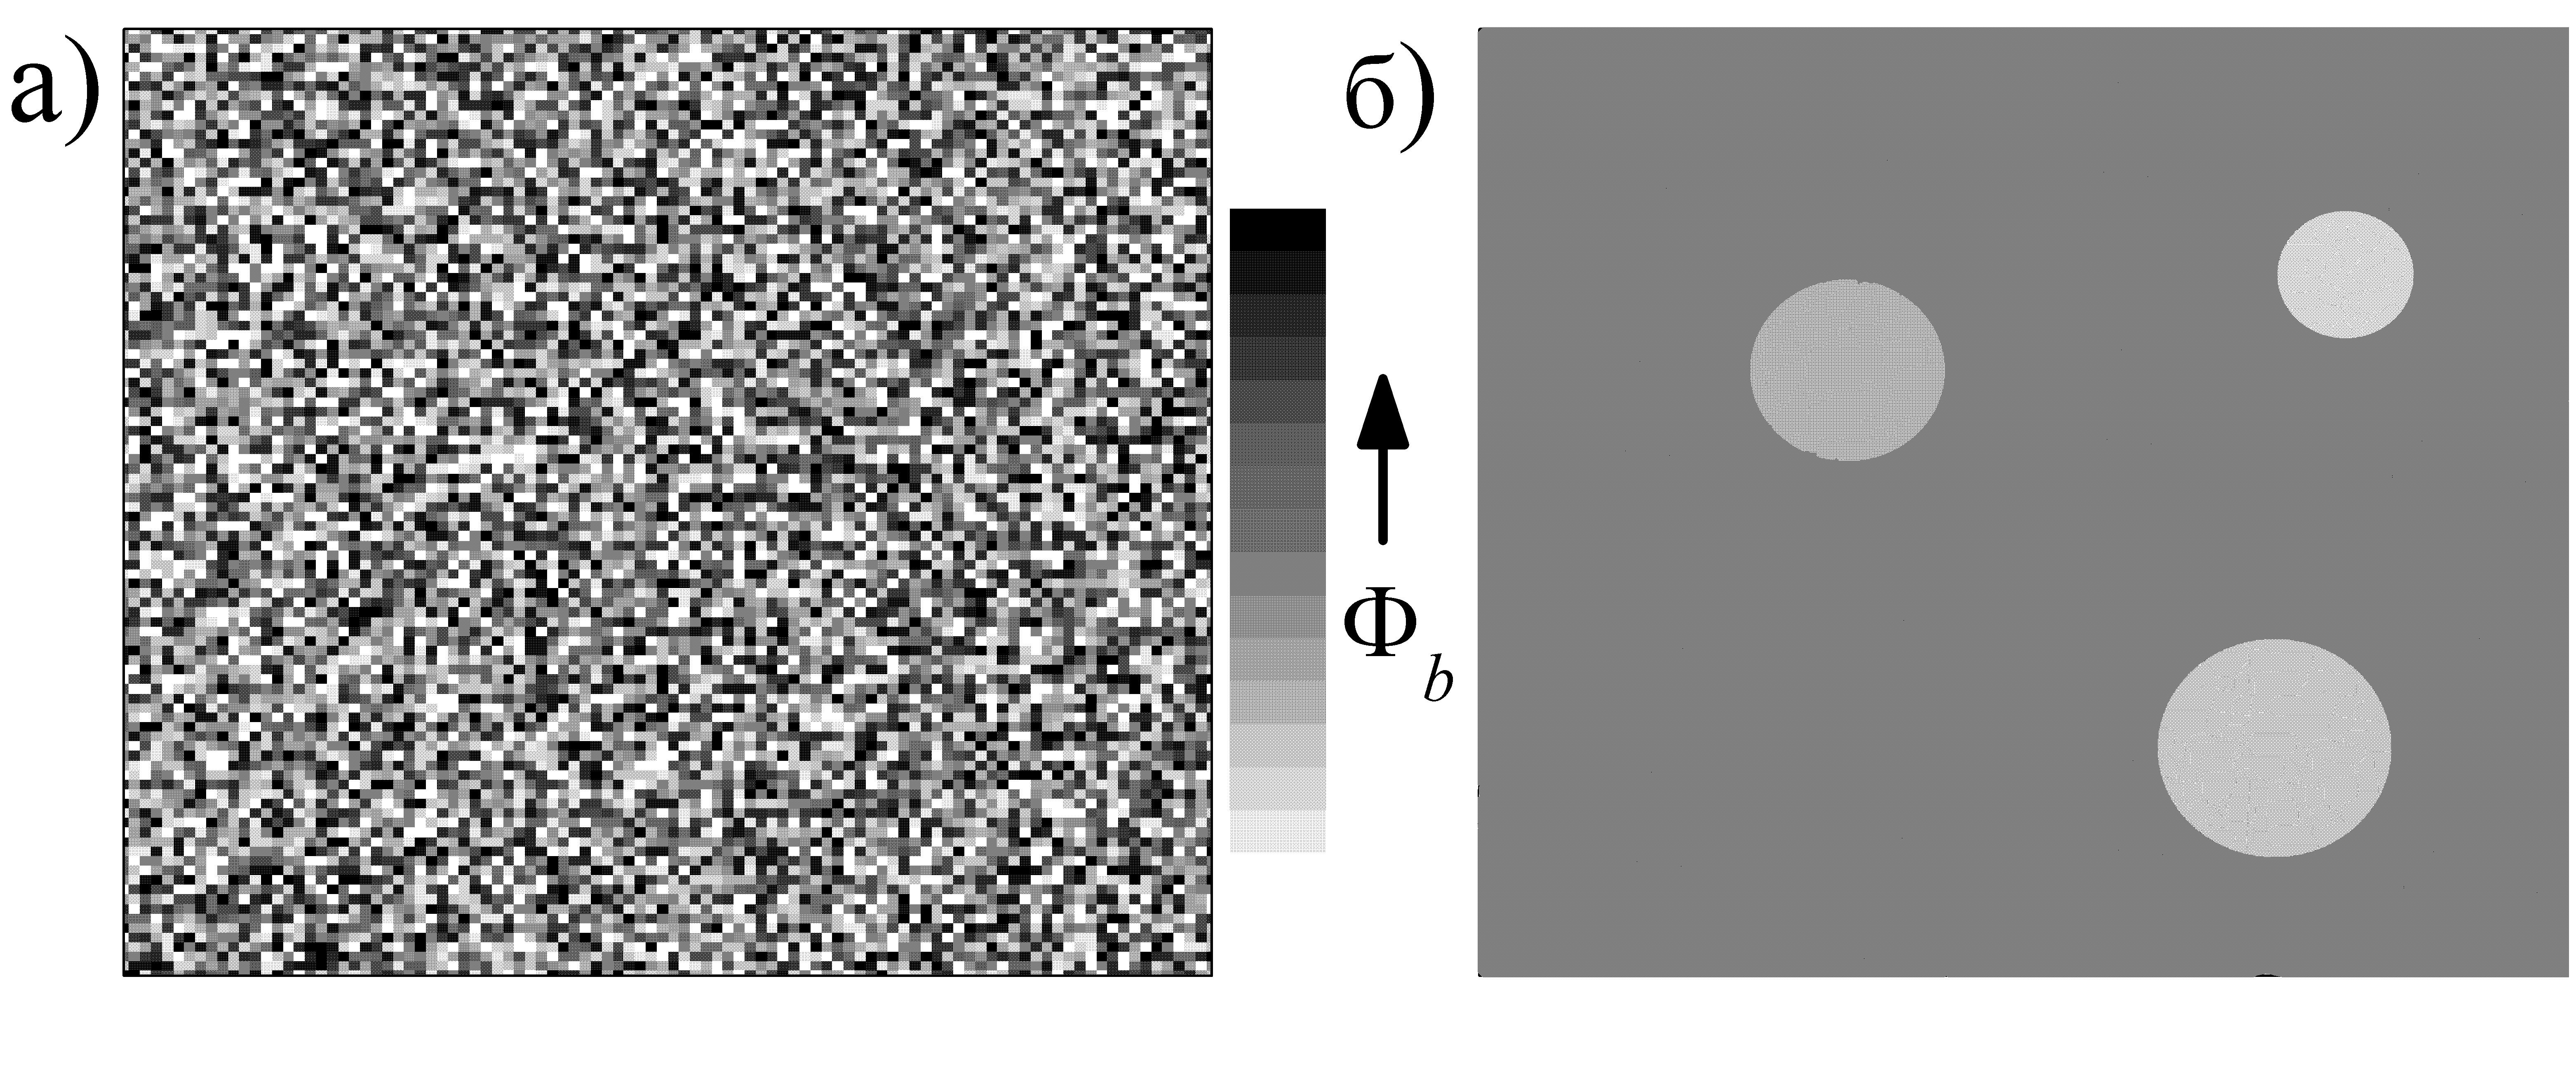
\includegraphics[width=0.9\textwidth]{figFbModel}
\caption{\label{figFbModel}
Моделі неоднорідного по площі контакту МН:
а --- ВБШ визначається розподілом Гауса;
б --- однорідний бар'єр з патчами.
}%
\end{figure}

Ця теорія передбачає,
що фактор неідеальності, який визначається за нахилом ВАХ, і ВБШ, розрахована за допомогою виразу (\ref{eqFb:TE}),
пов'язані з $\rho_2$ та $\rho_3$ і
$\Phi_{b}^0$ та $\sigma_{\Phi0}$, відповідно \cite{Werner,Tascioglu2010,Yildirim2010,Mamor,Soylu}:
\begin{equation}\label{eqNidT}
  \frac{1}{n_\mathrm{id}}=-\rho_2+\frac{q\rho_3}{2kT}\,,
\end{equation}
\begin{equation}\label{eqFb0T}
\Phi_b=\Phi_b^0-\frac{q\sigma^2_{\Phi0}}{2kT}.
\end{equation}

Відповідно до іншої моделі неоднорідного контакту Шотки \cite{Sullivan,Tung:PhysRev,Tung:MSE,Tung:ApplPhysRev}, ВБШ вважається однаковою на всій границі МН,
окрім невеликих за площею ділянок (так званих патчів), де значення ВБШ менше --- Рис.~\ref{figFbModel},б.
Ділянки можуть відрізнятися між собою площею та висотою бар'єру, причому відповідний характерний параметр описується розподілом Гауса.

В ряді робіт \cite{Iucolano2007JAP, Iucolano2007APL} показано, що ці теорії можуть бути використані сумісно,
причому за наявності патчів також має виконуватися співвідношення (\ref{eqFb0T}),
причому величина $\Phi_b^0$ має зміст ВБШ за межами патчів (в однорідній області),
а $\sigma_{\Phi0}$ пов'язаний з розподілом параметрів патчів.
Крім того, показано \cite{Sullivan,Tung:PhysRev,Iucolano2007JAP, Iucolano2007APL}, що при наявності неоднакових патчів
температурна залежність фактору неідеальності має описуватися виразом (\ref{eqN_T:TE}), причому
\begin{equation} \label{eqN_T0}
T_0=\frac{q\sigma_{\Phi0}^2}{3kV_{bb}}\,,
\end{equation}
де
$V_{bb}=(\Phi_b^0-V_n-V)$ --- вигин зон напівпровідника поблизу контакту.

Зауважимо, що підхід, який передбачає  врахування неоднорідності
інтерфейсної границі дуже широко використовується  для аналізу ВАХ різноманітних структур з контактом Шотки
\cite{Soylu,GELCZUK2014,Mohan,Yildirim2010,JYOTHI2015,DURMUS2014,KHURE2015,OZAVCI2013,Cetin2005,Karatas:2006NIMA,Sarpatwari,
Tascioglu2010, Yildirim2010, Mamor, Iucolano2007JAP, Iucolano2007APL,Li2016}.

Залежності, побудовані відповідно до виразів (\ref{eqNidT}) та (\ref{eqFb0T}) наведені на Рис.\ref{figFbNT1_SDA}.
Видно, що дійсно спостерігається лінійна залежність,
правда в двох окремих температурних діапазонах $T=(130\div220)$~К та $T=(230\div330)$~К.
Визначені шляхом лінійної апроксимації величини $\Phi_{b}^0$, $\sigma_{\Phi0}$, $\rho_2$ та $\rho_3$ для кожного з діапазонів
наведено в Таблиці~\ref{tabPar:SSDA}.

\begin{figure}
\center
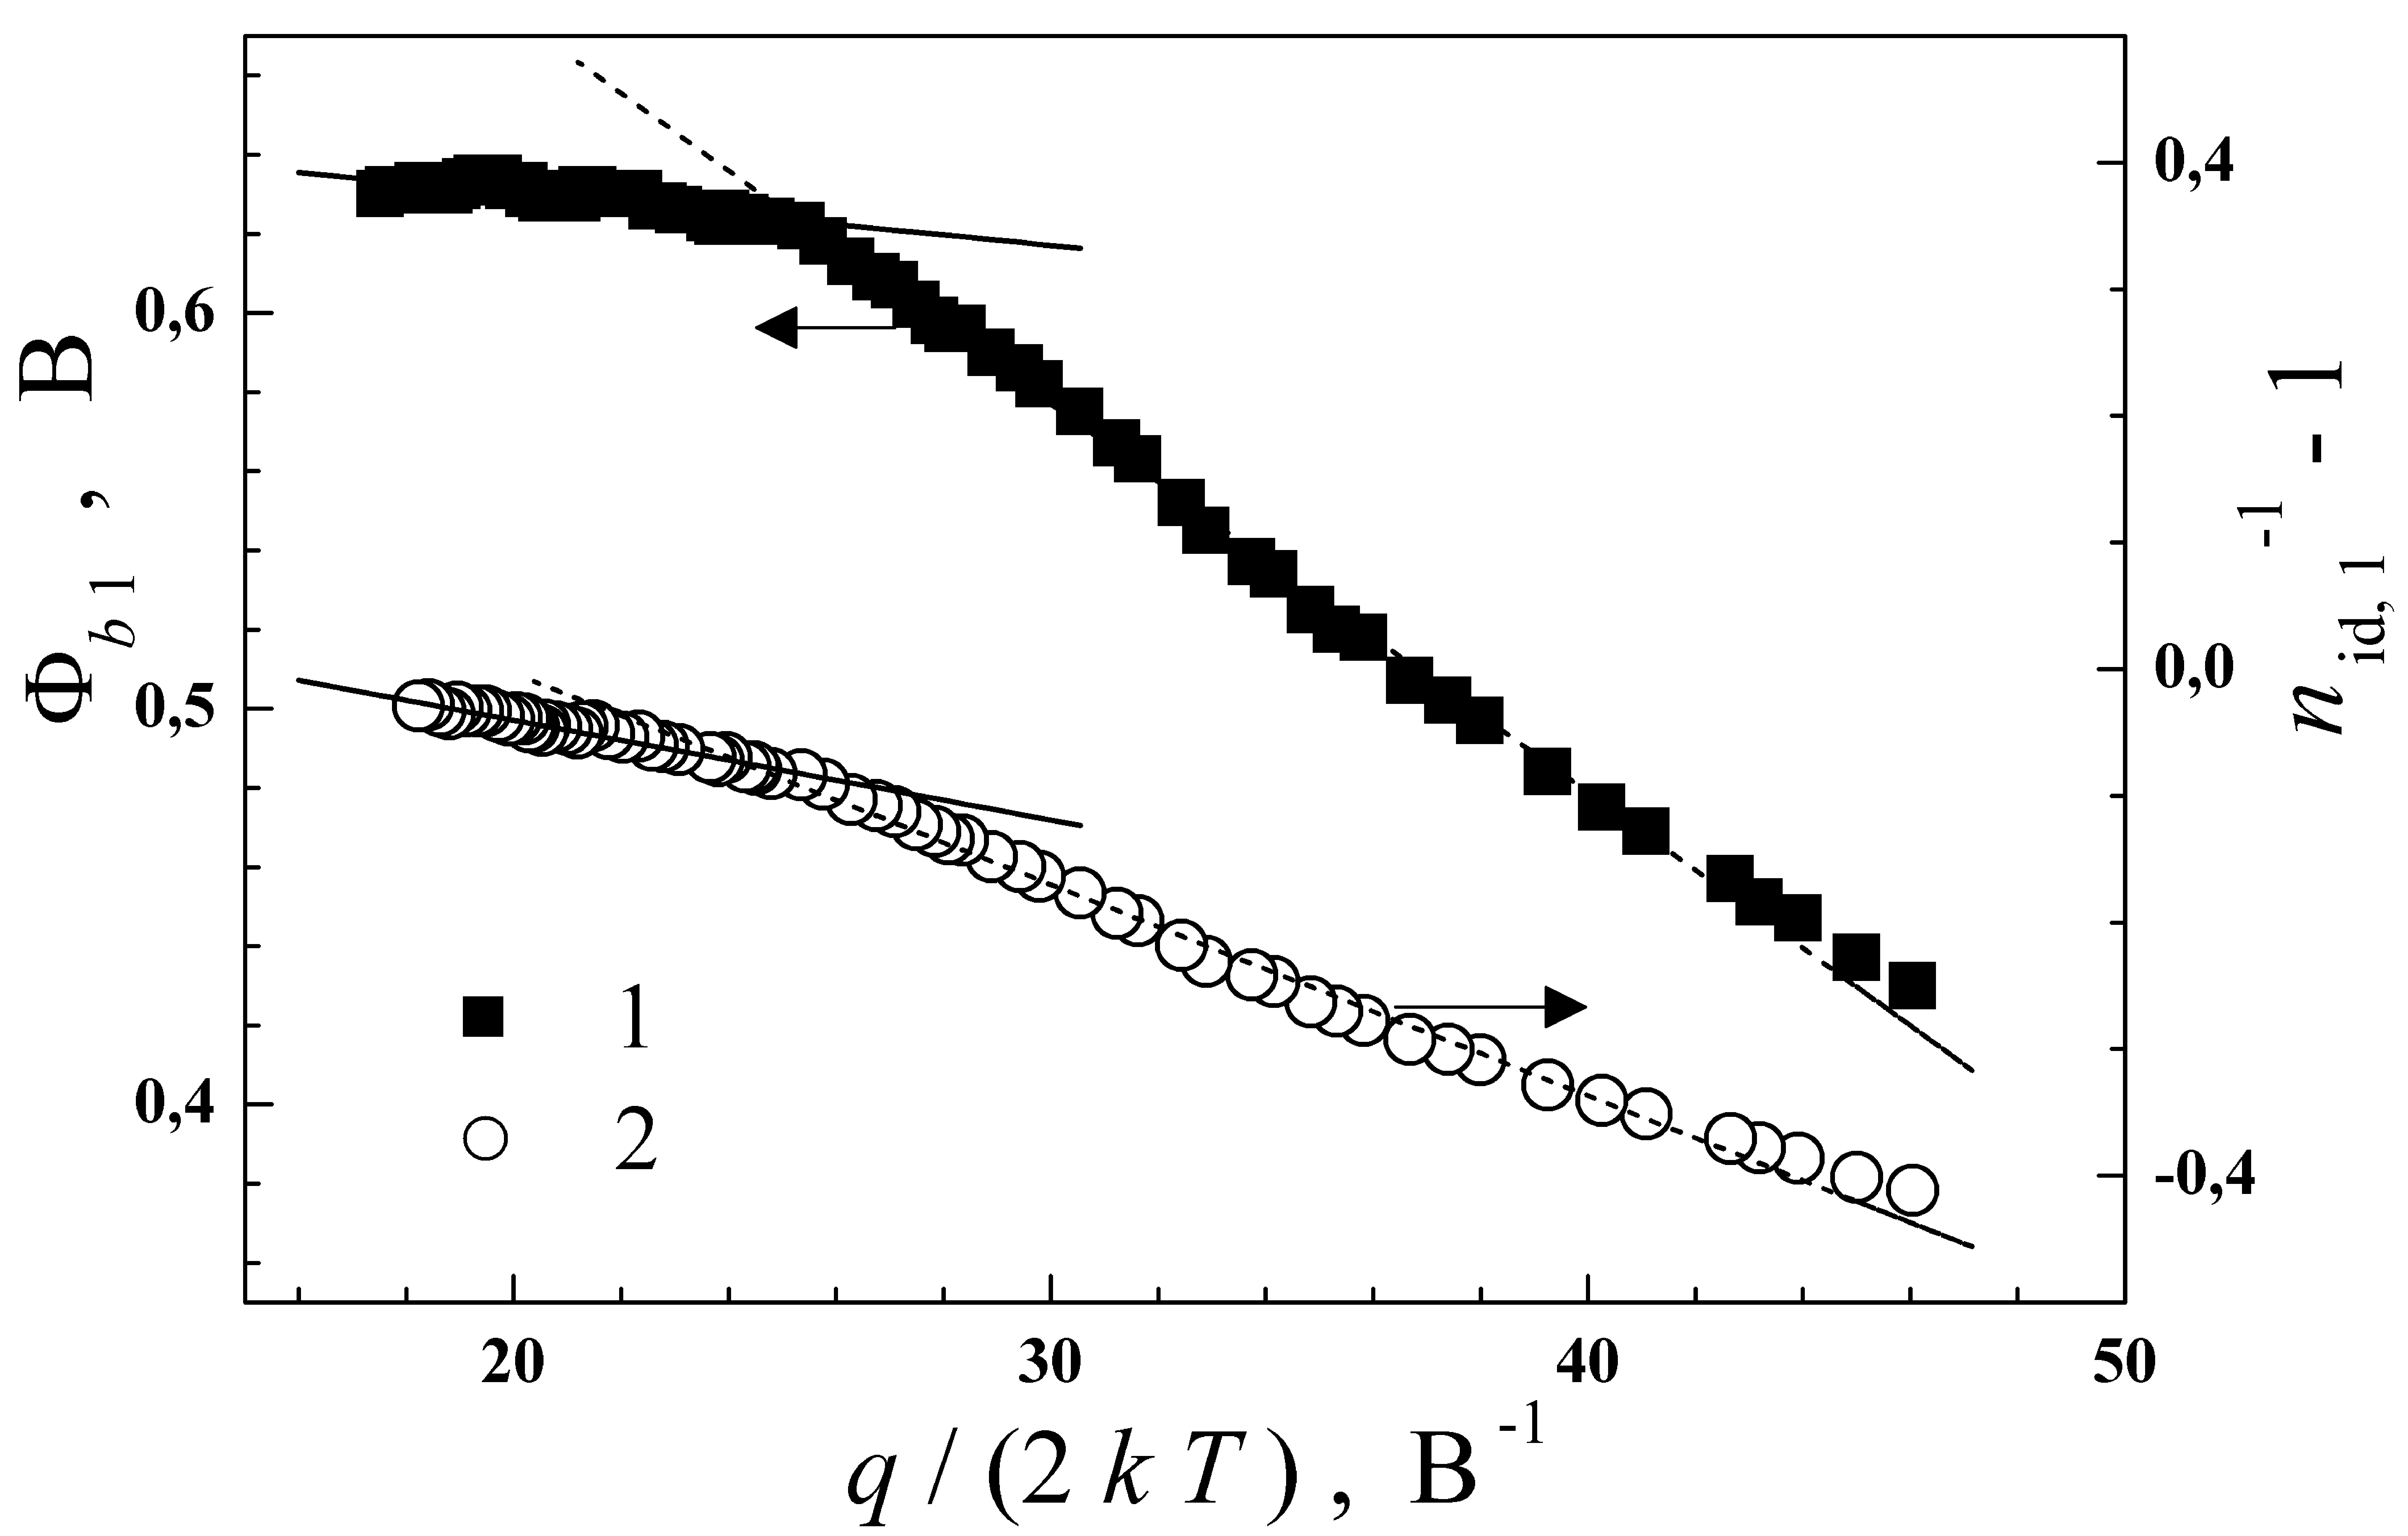
\includegraphics[width=0.7\textwidth]{figFbNT1_SDA}
\caption{\label{figFbNT1_SDA}
Залежності величин $\Phi_{b1}$ (крива 1) та $n_{\mathrm{id},1}^{-1}-1$ (крива 2) від оберненої температури.
Прямі --- лінійна апроксимація у діапазонах $T=(130\div220)$~К (суцільна) та $T=(230\div330)$~К (пунктир).
}%
\end{figure}

Використовуючи вираз (\ref{eqN_T0}) та значення $V_{bb}\simeq0.53$~В, $\Phi_{B\!T}^0\simeq0.663$~В, $\sigma_\Phi\simeq0.04$~В
була розраховане значення $T_{0,teor}\approx11$~К, яке очікується в рамках моделі контакту Шотки з локальними неоднорідностями
для температурного діапазону $(230\div330)$~К.
Ця величина досить близька до значення $T_{0,exp}\approx12$~К, отриманого експериментально (Рис.~\ref{figNT_SDA}) у цьому ж діапазоні.
Ще одним аргументом на користь того, що струм $I_1$ може бути описаний в рамках моделі ТЕ через неоднорідний контакт є якісний збіг
поведінки $n_{\mathrm{id},1}$ при низьких температурах (Рис.~\ref{figNT_SDA}) з очікуваною теоретично (\cite[Fig.11(b)]{Tung:PhysRev}).


У роботах  \cite{Tung:PhysRev,Sarpatwari,Schmitsdorf} показано, що для випадку
контакту з локальними неоднорідностями залежність між отриманими з аналізу ВАХ величинами $\Phi_b$ та $n_\mathrm{id}$ має бути лінійною,
причому $\Phi_{b}^0=\Phi_{b}+\Delta\Phi_b^\mathrm{IF}$ при $n=n_\mathrm{id}^\mathrm{IF}$
де $n_\mathrm{id}^\mathrm{IF}$ ---  величина фактору неідеальності з врахуванням впливу сил зображення,
$\Delta\Phi_b^\mathrm{IF}$ --- зниження бар'єру внаслідок дії сил зображення,
згідно з \cite{Sarpatwari}
\begin{equation}\label{eqN:IF}
n_\mathrm{id}^\mathrm{IF}\approx 1+\frac14\left[\frac{q^3N_d}{8\pi^2\varepsilon^2\varepsilon_0^2V^3_{bb}}\right]^{1/4},
\end{equation}
\begin{equation}\label{eqFb:IF}
\Delta\Phi_b^\mathrm{IF}\approx \left(\frac{q^3N_d\,V_{bb}}{8\pi^2\varepsilon^2\varepsilon_0^2}\right)^{1/4}.
\end{equation}
На залежності $\Phi_{b1}$ від $n_{\mathrm{id},1}$ (Рис.~\ref{figFbN_SDA}), як і в попередній випадках,
спостерігаються дві лінійні області зі зламом при $T\sim225$~К.
Шляхом екстраполяції отримано, що $\Phi_b^0$ дорівнює 0,646~В 0,64~В при низьких та високих температурах, відповідно.
Похибки визначення наведено в Таблиці~\ref{tabPar:SSDA}.
Зауважимо, що, згідно з \cite{Sarpatwari,Schmitsdorf},
при зниженні температури зростає роль проходження струму через патчі і, хоча лінійність між  $\Phi_b$ та $n_\mathrm{id}$ зберігається,
екстрапольоване значення ВБШ не буде дорівнювати висоті бар'єру в однорідній області.
На нашу думку, саме цим пояснюється відмінність величини $\Phi_b$, визначеної за залежністю
$\Phi_b=f(n_\mathrm{id})$ в низькотемпературному діапазоні, від інших,
отриманих для $T=(130\div220)$~К з використанням моделі неоднорідного бар'єру (див.~Таблиці~\ref{tabPar:SSDA}).

\begin{figure}
\center
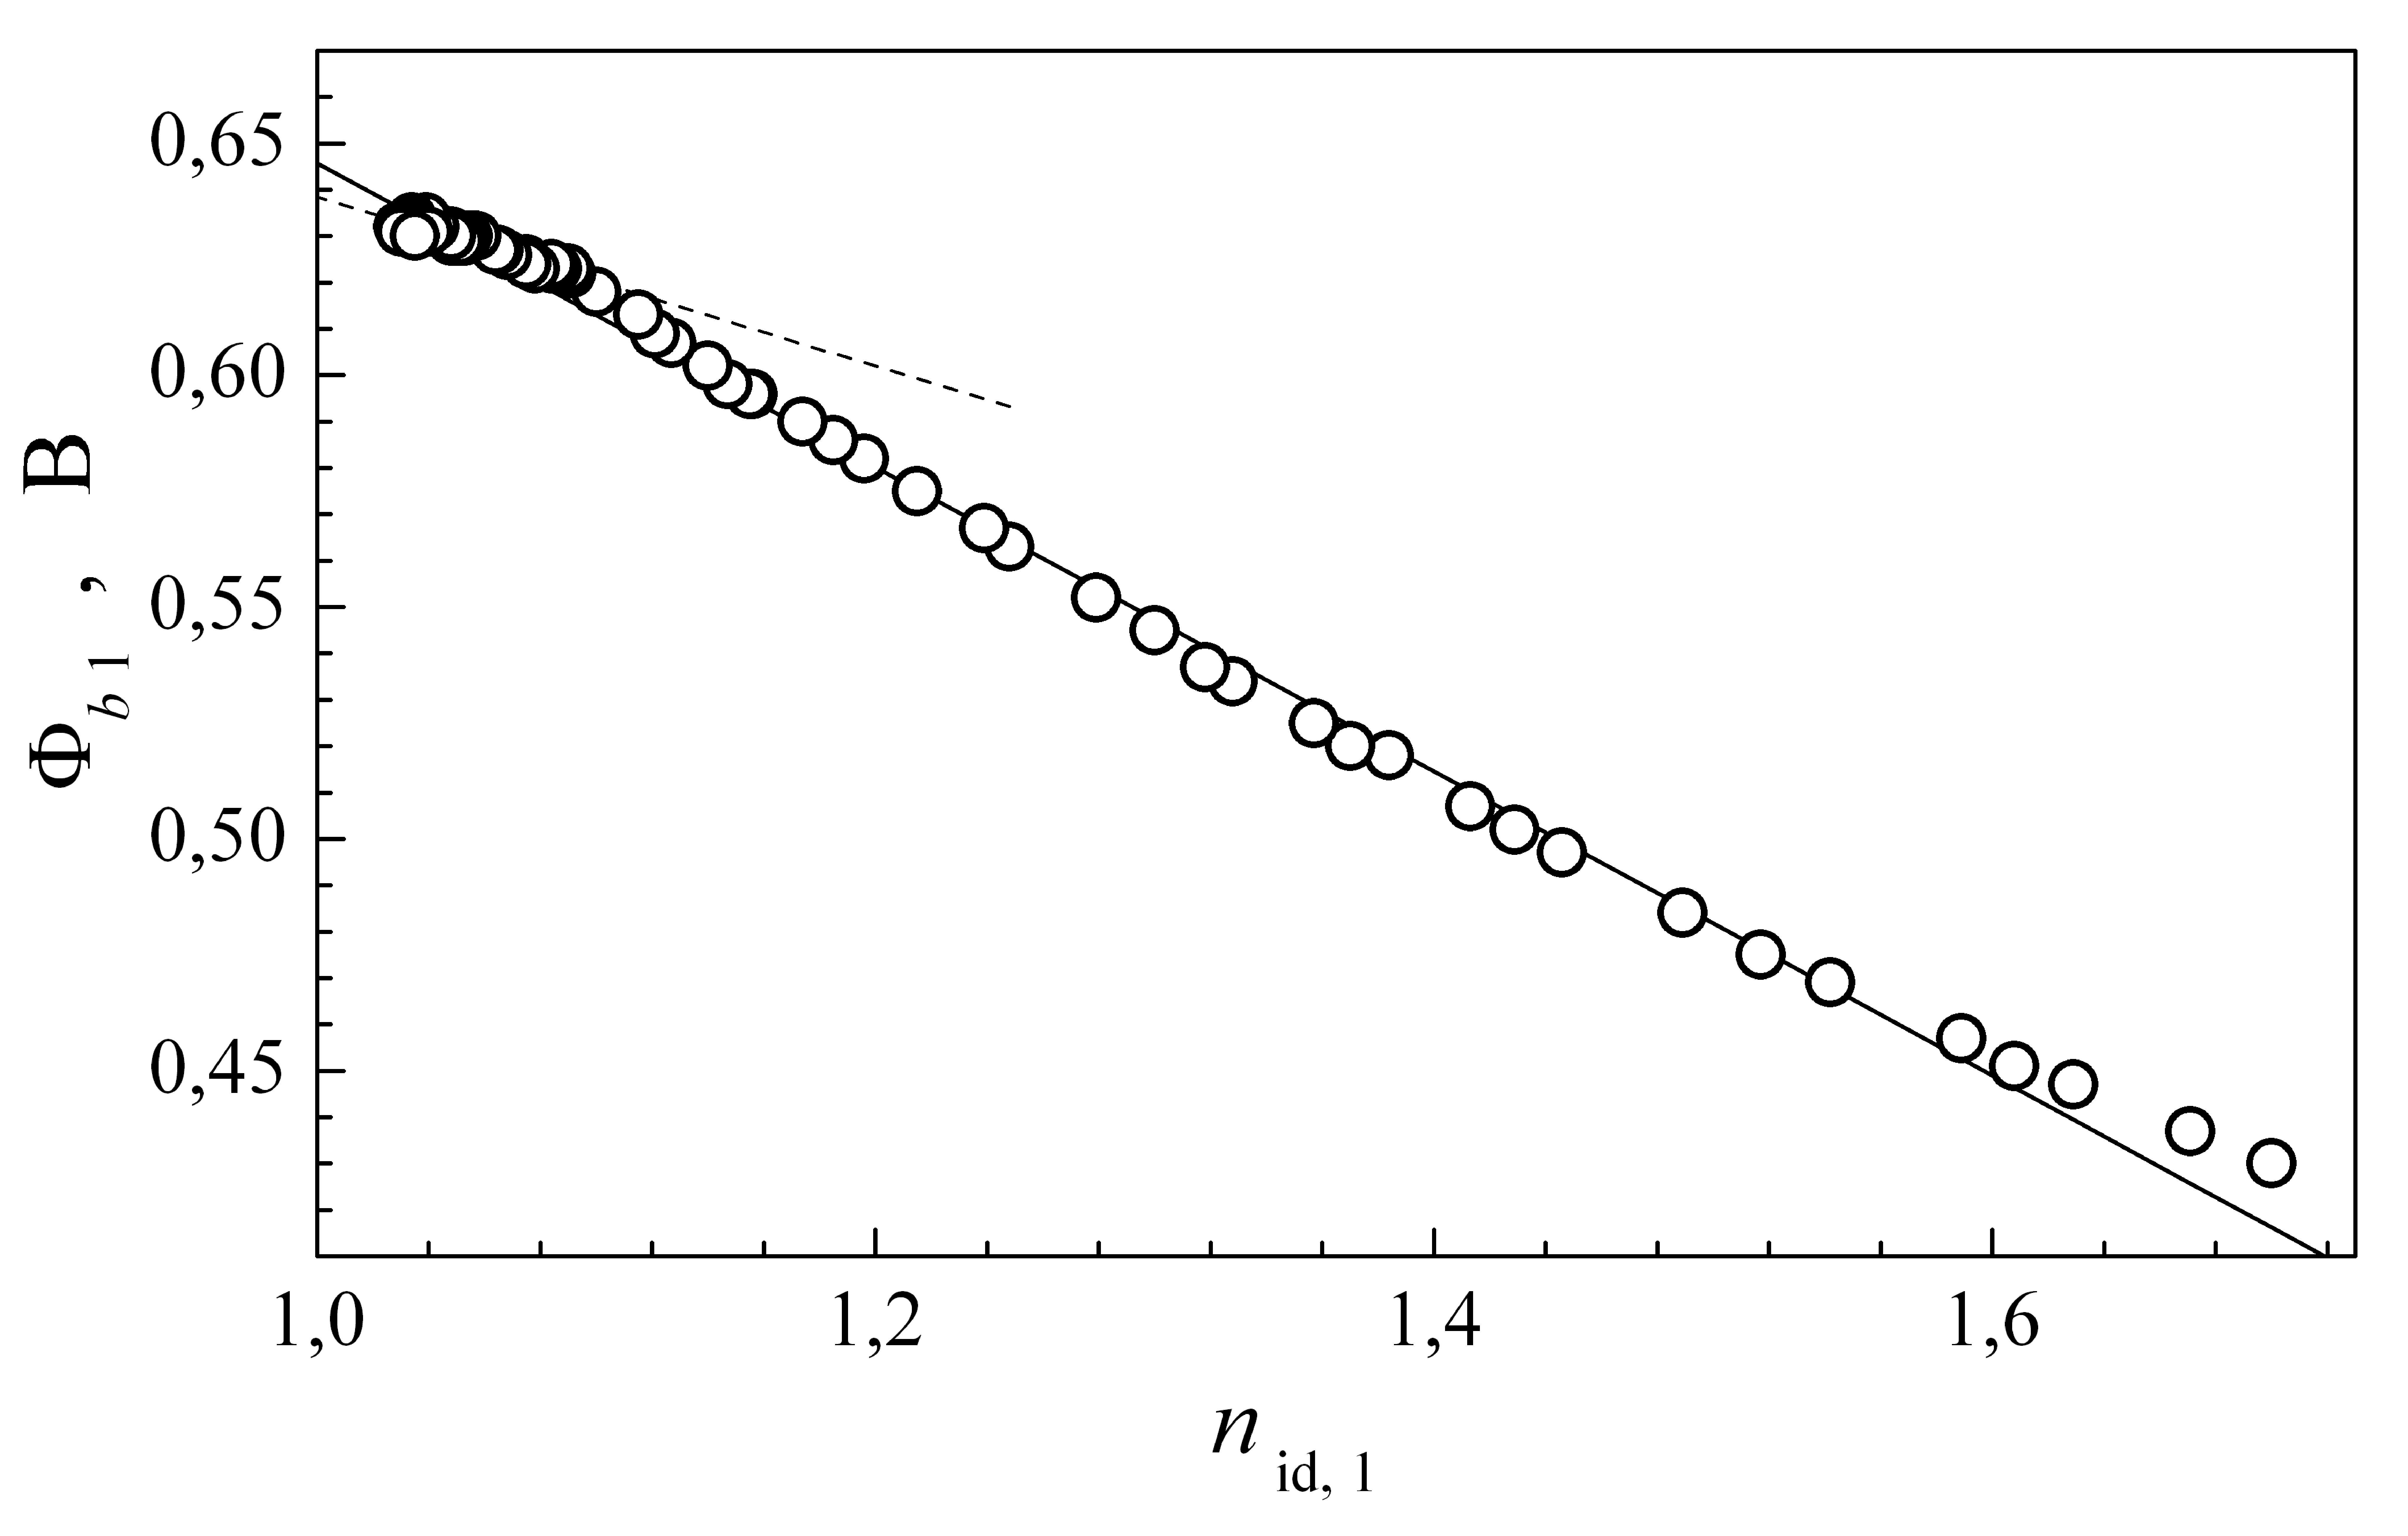
\includegraphics[width=0.7\textwidth]{figFbN_SDA}
\caption{\label{figFbN_SDA}
Залежність ВБШ від фактору неідеальності для високотемпературної компоненти струму $I_1$.
Прямі --- лінійна апроксимація у діапазонах $T=(130\div220)$~К (суцільна) та $T=(230\div330)$~К (пунктир).
}%
\end{figure}

У випадку неоднорідного бар'єру Шотки стала Річардсона може бути визначена за
допомогою модифікованої залежності Річардсона \cite{Tascioglu2010old,Yildirim2010}:
\begin{equation} \label{eqRich:Mod}
\ln\left(\frac{I_s}{T^2}\right)-\left(\frac{q^2\sigma_{\Phi0}^2}{2k^2T^2}\right)=\ln(AA^*)-\frac{q\Phi_b^0}{kT}.
\end{equation}

Відповідні графіки, побудовані з використанням отриманих значень $\sigma_{\Phi,0}$ показано на Рис.~\ref{figRichM_SDA}.
Лінійна апроксимація отриманих кривих у температурних діапазонах, відповідних тим, де були визначені стандартні відхилення
дозволили оцінити середнє значення ВБШ та сталу Річардсона.
Відповідні дані наведено в Таблиці~\ref{tabPar:SSDA}.
Зауважимо, що величини $A^*$, отримані в різних діапазонах температур в межах похибок збігаються
\begin{enumerate}[label=\asbuk*),leftmargin=0em,itemindent=1.5em]
\item між собою;
\item з літературними даними.
\end{enumerate}


\begin{figure}
\center
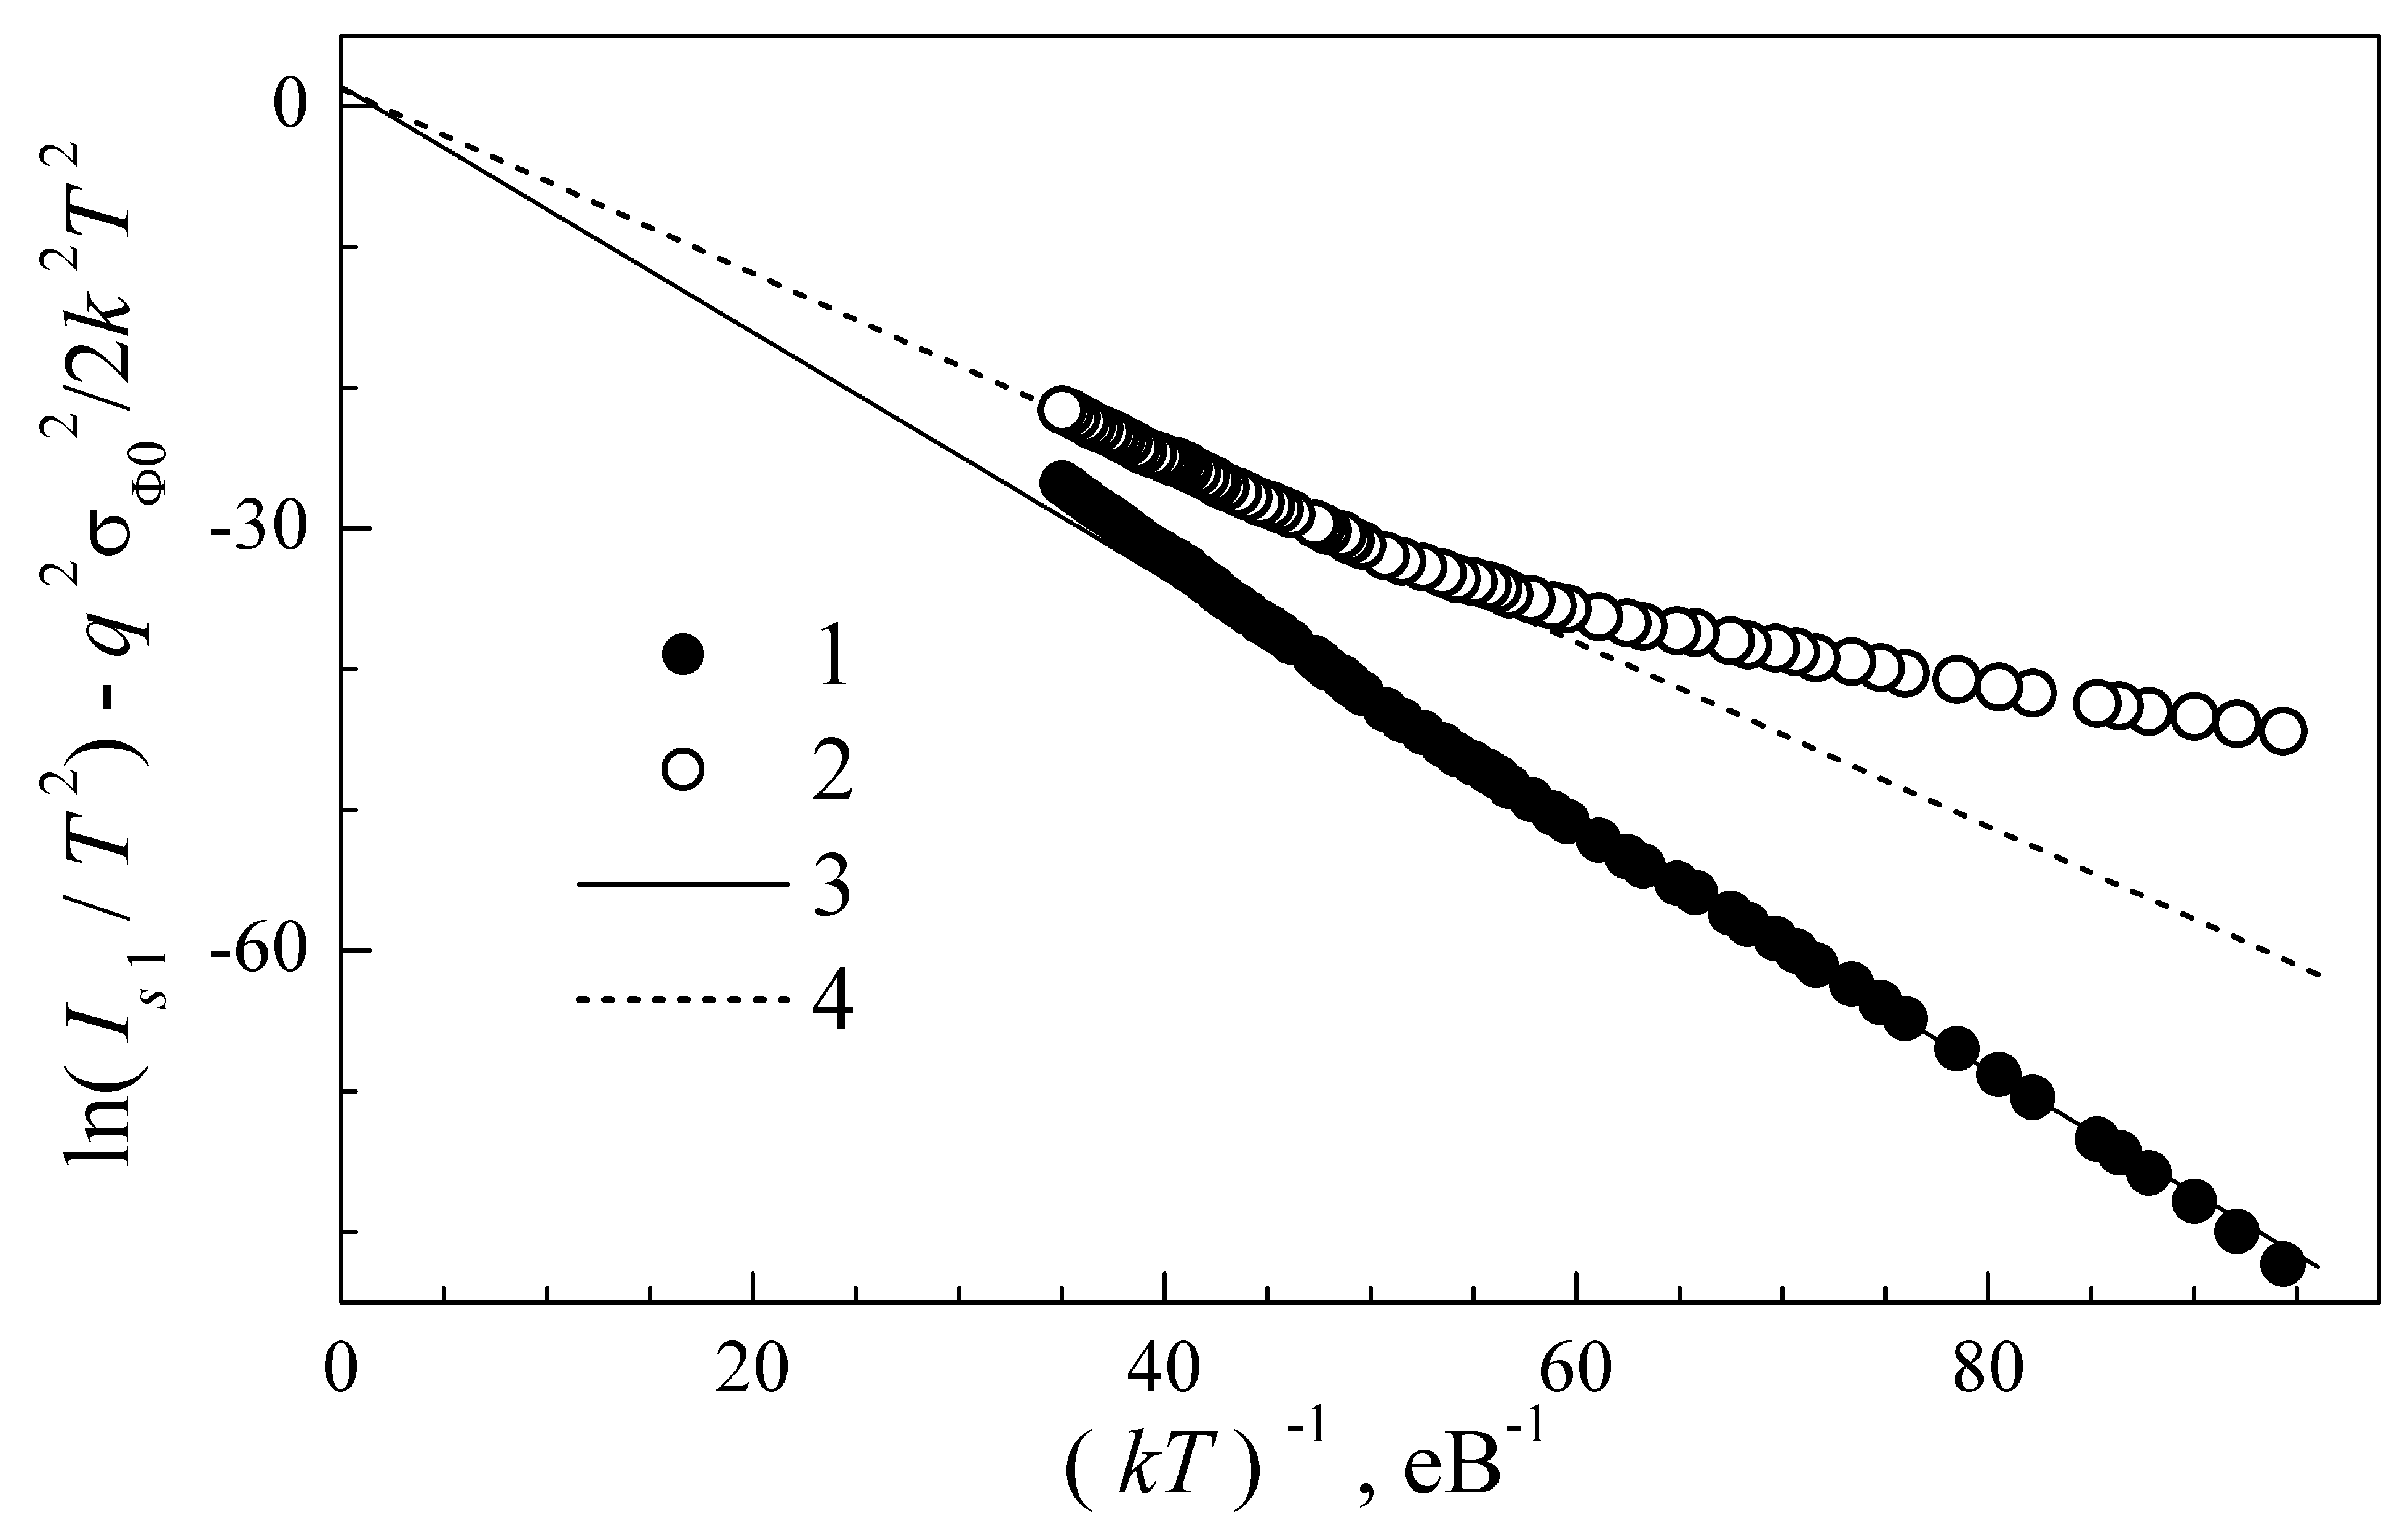
\includegraphics[width=0.9\textwidth]{figRichM_SDA}
\caption{\label{figRichM_SDA}
Модифіковані залежності Річардсона, розраховані за формулою (\ref{eqRich:Mod}) для $I_{s1}$.
$\sigma_{\Phi,0}$, В: 0,099 (крива 1) та 0,04 (2).
Прямі 3 та 4 --- лінійна апроксимація кривих 1 та 2 в діапазонах $T=(130\div220)$~К
та $T=(230\div330)$~К, відповідно.
}%
\end{figure}

В Таблиці~\ref{tabPar:SSDA} також наведено значення висоти бар'єру, визначене з ВФХ.
В цьому випадку  \cite{Rhoderick1988,Schroder2006}:
\begin{equation}\label{eqFbCV}
\Phi_{b,CV}=V_n+V_0+\frac{kT}{q},
\end{equation}
де
$V_0$ --- абсциса точки перетину з віссю напруг прямої, яка апроксимує залежність $1/C^2=f(V)$ (див. Рис.~\ref{figCV}).
Зазначимо, що визначена таким способом ВБШ має перевищувати величину, отриману за допомогою ВАХ
\cite{Rhoderick1988,GELCZUK2014,Mohan,Cetin2005,Soylu,Yildirim2010,Karatas:2006NIMA}.
Це пов'язано з тим, що $\Phi_{b,CV}$ визначається, насамперед, вигином зон і на неї не впливають, наприклад,
наявність сил зображення чи квантово--механічне тунелювання носіїв \cite{Rhoderick1988,GELCZUK2014,Mohan}.
Більше того, неоднорідність контакту також не відображається на величині $\Phi_{b,CV}$ на відміну від ВБШ,
яка визначається за допомогою ВАХ \cite{Sullivan,Tung:PhysRev,GELCZUK2014,Mohan}.
За своєю поведінкою зі зміною температури $\Phi_{b,CV}$ нагадує ВБШ, визначену за умов плоских зон, наближаючись
до неї і за величиною \cite{Cetin2005,Soylu,Yildirim2010,Mohan}.
В нашому випадку спостерігається очікуване співвідношення $\Phi_{b,CV}>\Phi_b^0$ для всіх значень, отриманих
в наближенні неоднорідного контакту.

Таким чином, наведені вище результати свідчать про те, що струм $I_1$ може бути описаний в рамках моделі ТЕ через неоднорідний бар'єр.
Єдине, що потребує більш детальної уваги --- відмінність між значеннями $\Phi_b^0$ та  $\sigma_{\Phi}$ в різних температурних діапазонах,
яка напряму не передбачається в рамках теорії неоднорідного контакту.
Водночас подібна ситуація нерідко спостерігається експериментально, див., наприклад,
\cite{Tascioglu2010old,Yildirim2010,Mamor,Jiang:DGJap,JYOTHI2015,DURMUS2014,KHURE2015,OZAVCI2013,Tung:ApplPhysRev}.
Пов'язувалися подібні зміни  з домінуванням при низьких температурах інших, порівняно з ТЕ, механізмів перенесення заряду
(термопольова емісія, тунелювання чи рекомбінаційні процеси), фазовими перетвореннями в металі тощо.
Проте, на нашу думку, в даному випадку збіг  отриманих значень $A^*$ з літературними свідчить про застосовність саме теорії ТЕ.
Причиною зміни нахилів залежностей на Рис.~\ref{figFbNT1_SDA} та \ref{figRichM_SDA} може бути збільшення швидкості емісії електронів дефектами на границі МН.
Дійсно, звільнення рівнів окремих дефектів при $T\approx225$~K має стати причиною зменшення ВБШ, а також того,
що частина ділянок неоднорідності, в околі яких концентрація подібних дефектів підвищена, перестане бути зонами полегшеного проходження струму внаслідок ефективного захоплення дрейфуючих електронів пастками.
В результаті, у більш високотемпературному діапазоні $\sigma_{\Phi0}$ має зменшуватися, що і спостерігається на експерименті.
Інший варіант пояснення, який пропонується, зокрема, в роботі \cite{Tung:ApplPhysRev},
полягає в тому, що окрім патчів наявна додаткова неоднорідність інтерфейсу метал--напівпровідник.
Як правило, із ВАХ вдається визначити ВБШ для ділянок з меншим значенням $\Phi_b^0$ і лише при низькотемпературних вимірюваннях
нахил модифікованої залежності Річардсона дозволяє отримати інформацію про верхню границю розподілу висоти бар'єру.


Повернімось до струму $I_2$, який превалює при малих зміщеннях у низькотемпературній області.
В роботі~\cite{Tung:PhysRev} показано, що у випадку неоднорідного контакту такий додатковий, порівняно з $I_1$, струм
може з'являтися саме при низьких температурах внаслідок ефективного проходженню носіїв через патчі.
При цьому експериментальна залежність, показана на Рис.~\ref{figIV_SDA} дуже схожа на передбачену теоретично (див. Fig.6 в \cite{Tung:PhysRev}).
Крім того, у теорії очікується, що для відповідної ділянки ВАХ фактор неідеальності має значно перевищувати одиницю
і має спостерігатися суттєвий вплив послідовного опору.
Саме це і було виявлене в наших дослідженнях.
У випадку, коли струм через патчі визначається ТЕ, то, згідно з \cite{Sarpatwari, Tung:PhysRev},
\begin{equation}\label{eqIlowT}
I_s=f_pAA^*T^2\exp\left(-\frac{q\Phi_{b,p}}{kT}\right),
\end{equation}
де
$f_p$  --- множник, який враховує площу ділянок неоднорідності,
$\Phi_{b,p}$ --- ВБШ в області патчу.
Порівнюючи вирази (\ref{eqIlowT}) та (\ref{eqFb:TE}), можна
записати співвідношення між $\Phi_{b,p}$ та $\Phi_{b}$:
\begin{equation}\label{eqFbFbp}
\Phi_b=\Phi_{b,p}-\frac{kT}{q}\ln{f_p}\,.
\end{equation}
Як видно з рис.~\ref{figFbT_SDA}, величина $\Phi_{b2}$ дійсно є лінійною функцією температури.
Шляхом лінійної апроксимації експериментальних даних визначено, що $\Phi_{b,p}=(54\pm4)$~мВ,
$f_p=(8\pm1)\times10^{-13}$.
Таким чином, додатковий струм, який виникає при низьких температурах, також може бути пояснений з точки
зору моделі неоднорідного контакту Шотки.

\subsection{Перенесення заряду при зворотному зміщенні}

Приклади зворотних гілок ВАХ структур SSDA, виміряних при різних температурах, наведено на рис.~\ref{figIV_SDAr}.
Видно, що на представлених характеристиках не спостерігається насичення величини зворотного струму $I_R$.
Це свідчить про те,
що характеристики не можуть бути описані в рамках моделі ТЕ через бар'єр з постійною для певної температури висотою.
Зауважимо, що подібна поведінка (відсутність насичення зворотного струму) є типовою
практично для всіх реальних ДШ.
Це явище навіть отримало окрему назву --- <<м'які>> (<<soft>>) зворотні характеристики.

Зростання струму при підвищенні температури залежить від зміщення:
при збільшенні зворотної напруги $V_R$ температурна залежність $I_R$ послаблюється.
З метою визначення механізму перенесення заряду були побудовані залежності величини струму при певному значенні напруги від температури,
представлені на Рис.~\ref{figIT_SDAr}.
З рисунка видно, що
\begin{enumerate}[label=\asbuk*),leftmargin=0em,itemindent=1.5em]
\item при аналізі зворотних ВАХ також, як і для прямих гілок, доцільно розглядати два температурних піддіапазони $(130\div220)$~К та $(230\div330)$~К;
\item при зворотному зміщенні перенесення заряду забезпечується завдяки декільком механізмам.
\end{enumerate}



\begin{figure}
\center
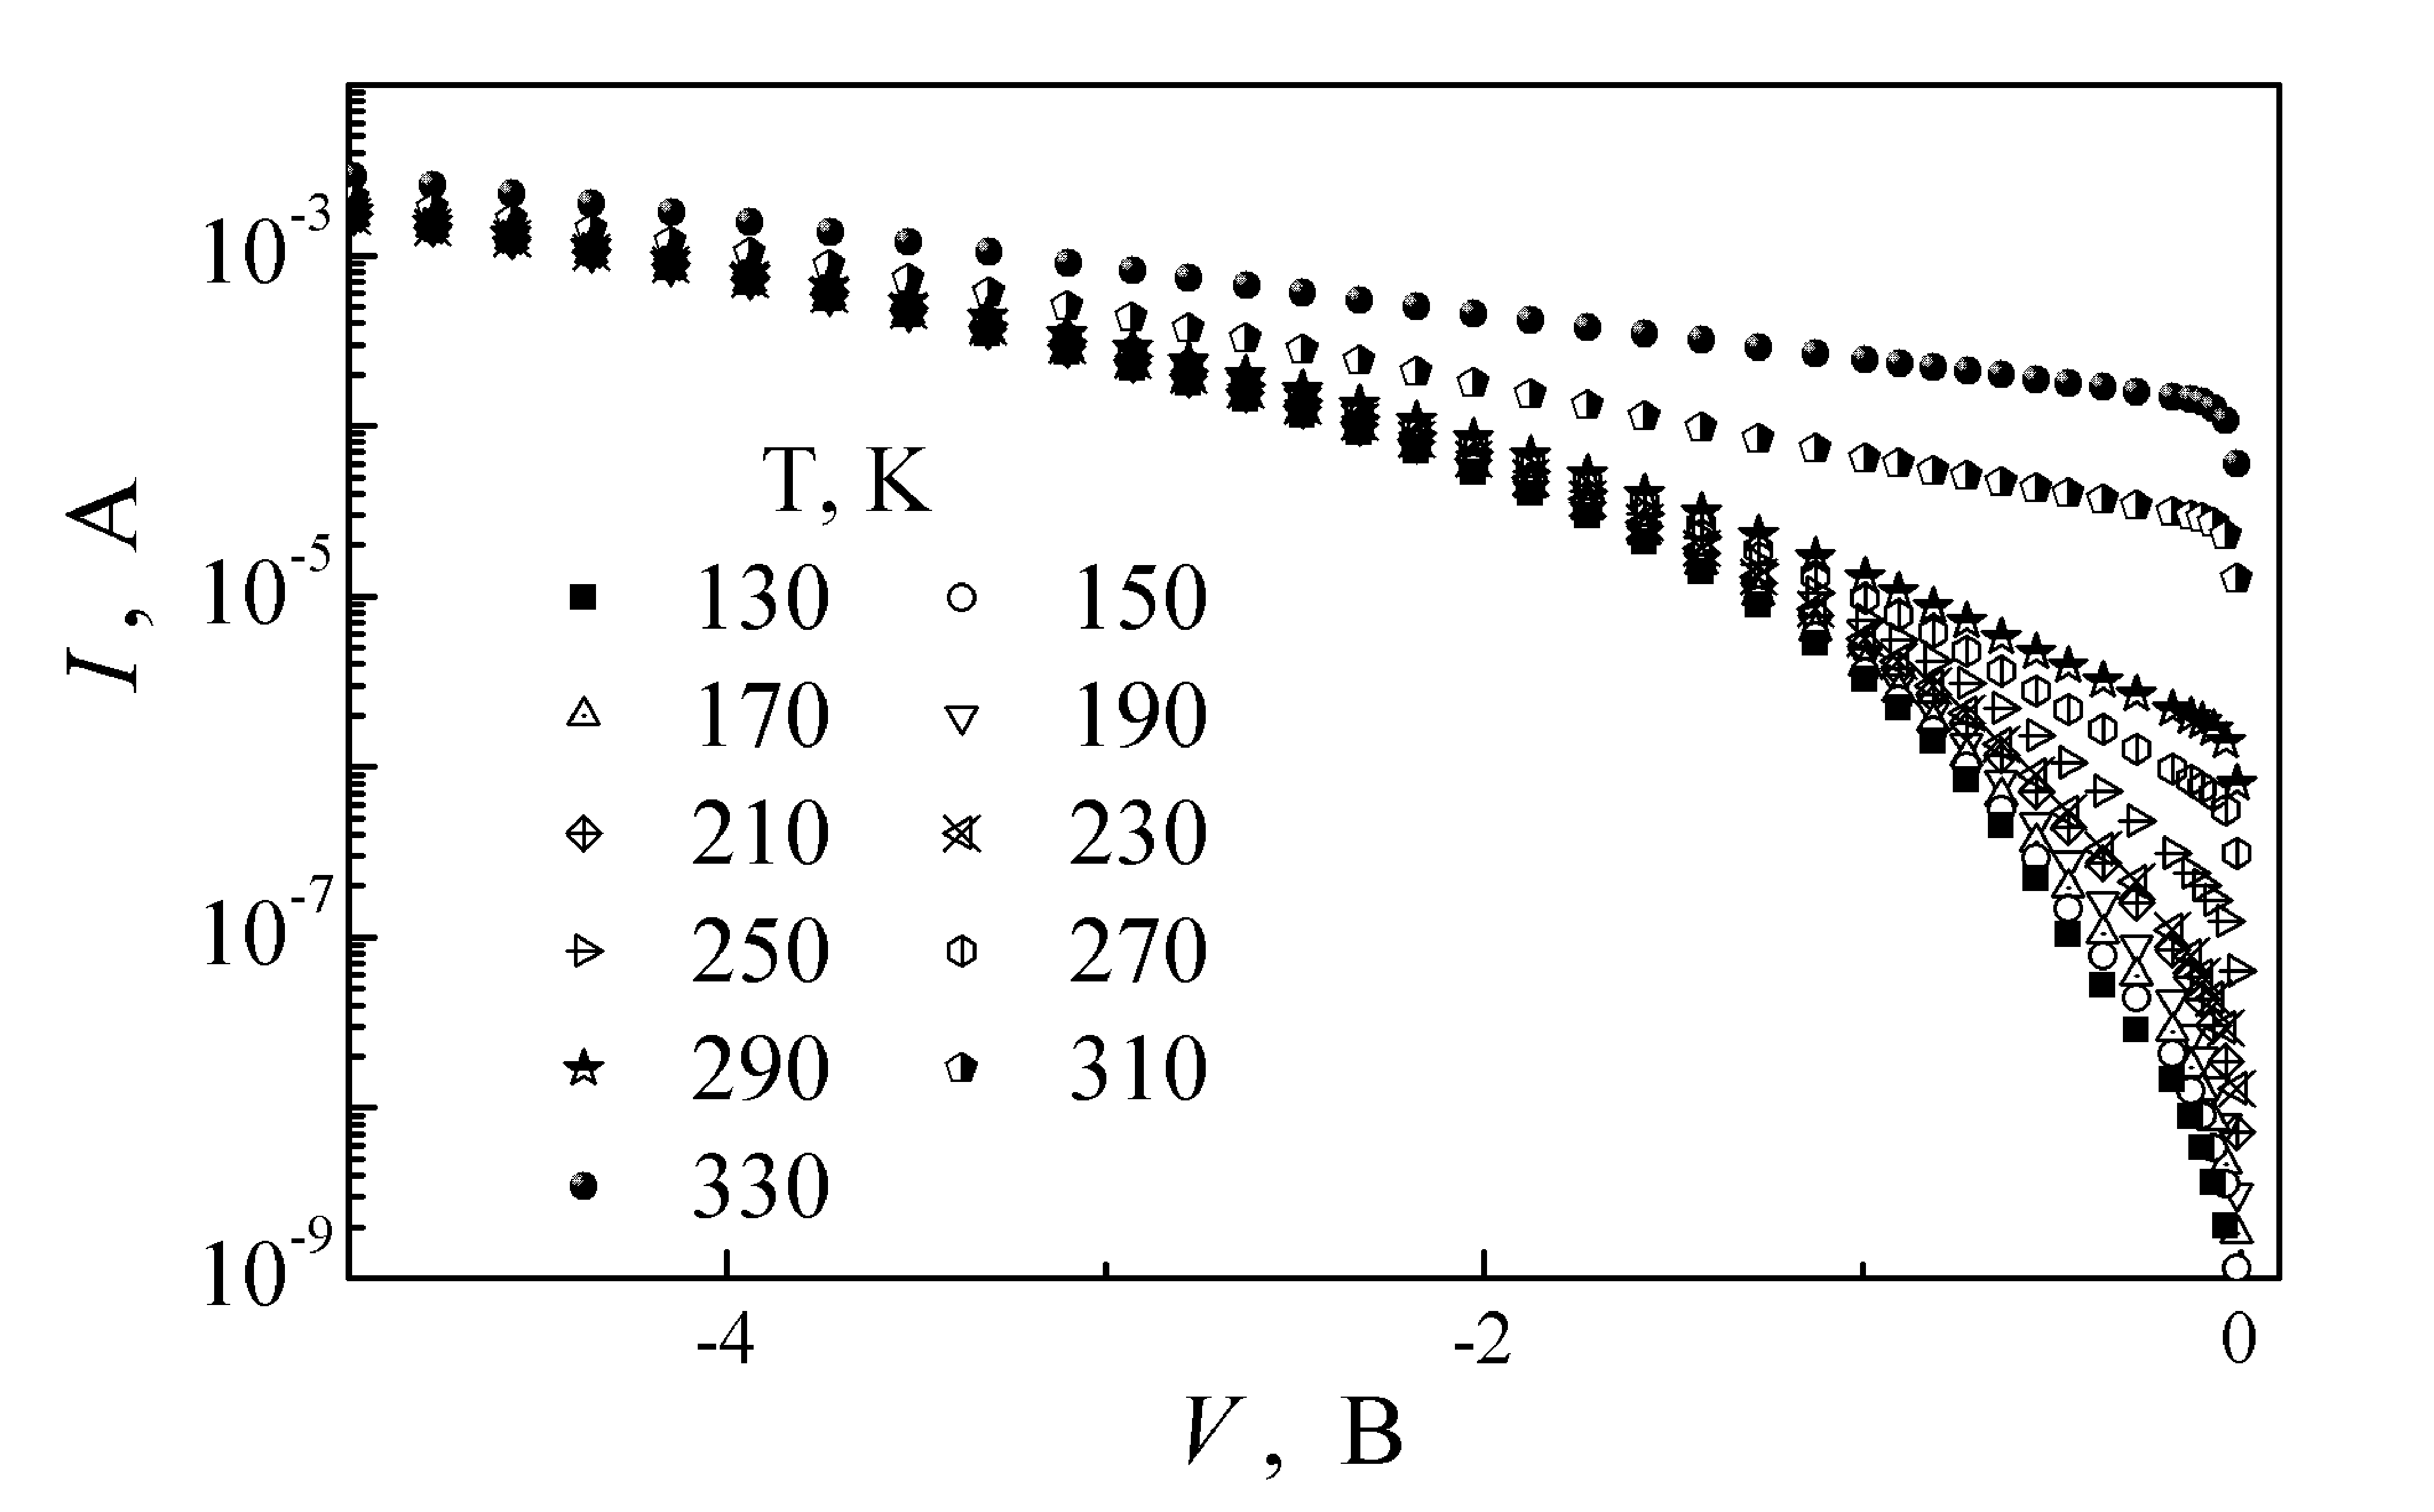
\includegraphics[width=0.8\textwidth]{figIV_SDAr}
\caption{\label{figIV_SDAr}
Зворотні гілки ВАХ структур SSDA при різних температурах.
}%
\end{figure}


\begin{figure}
\center
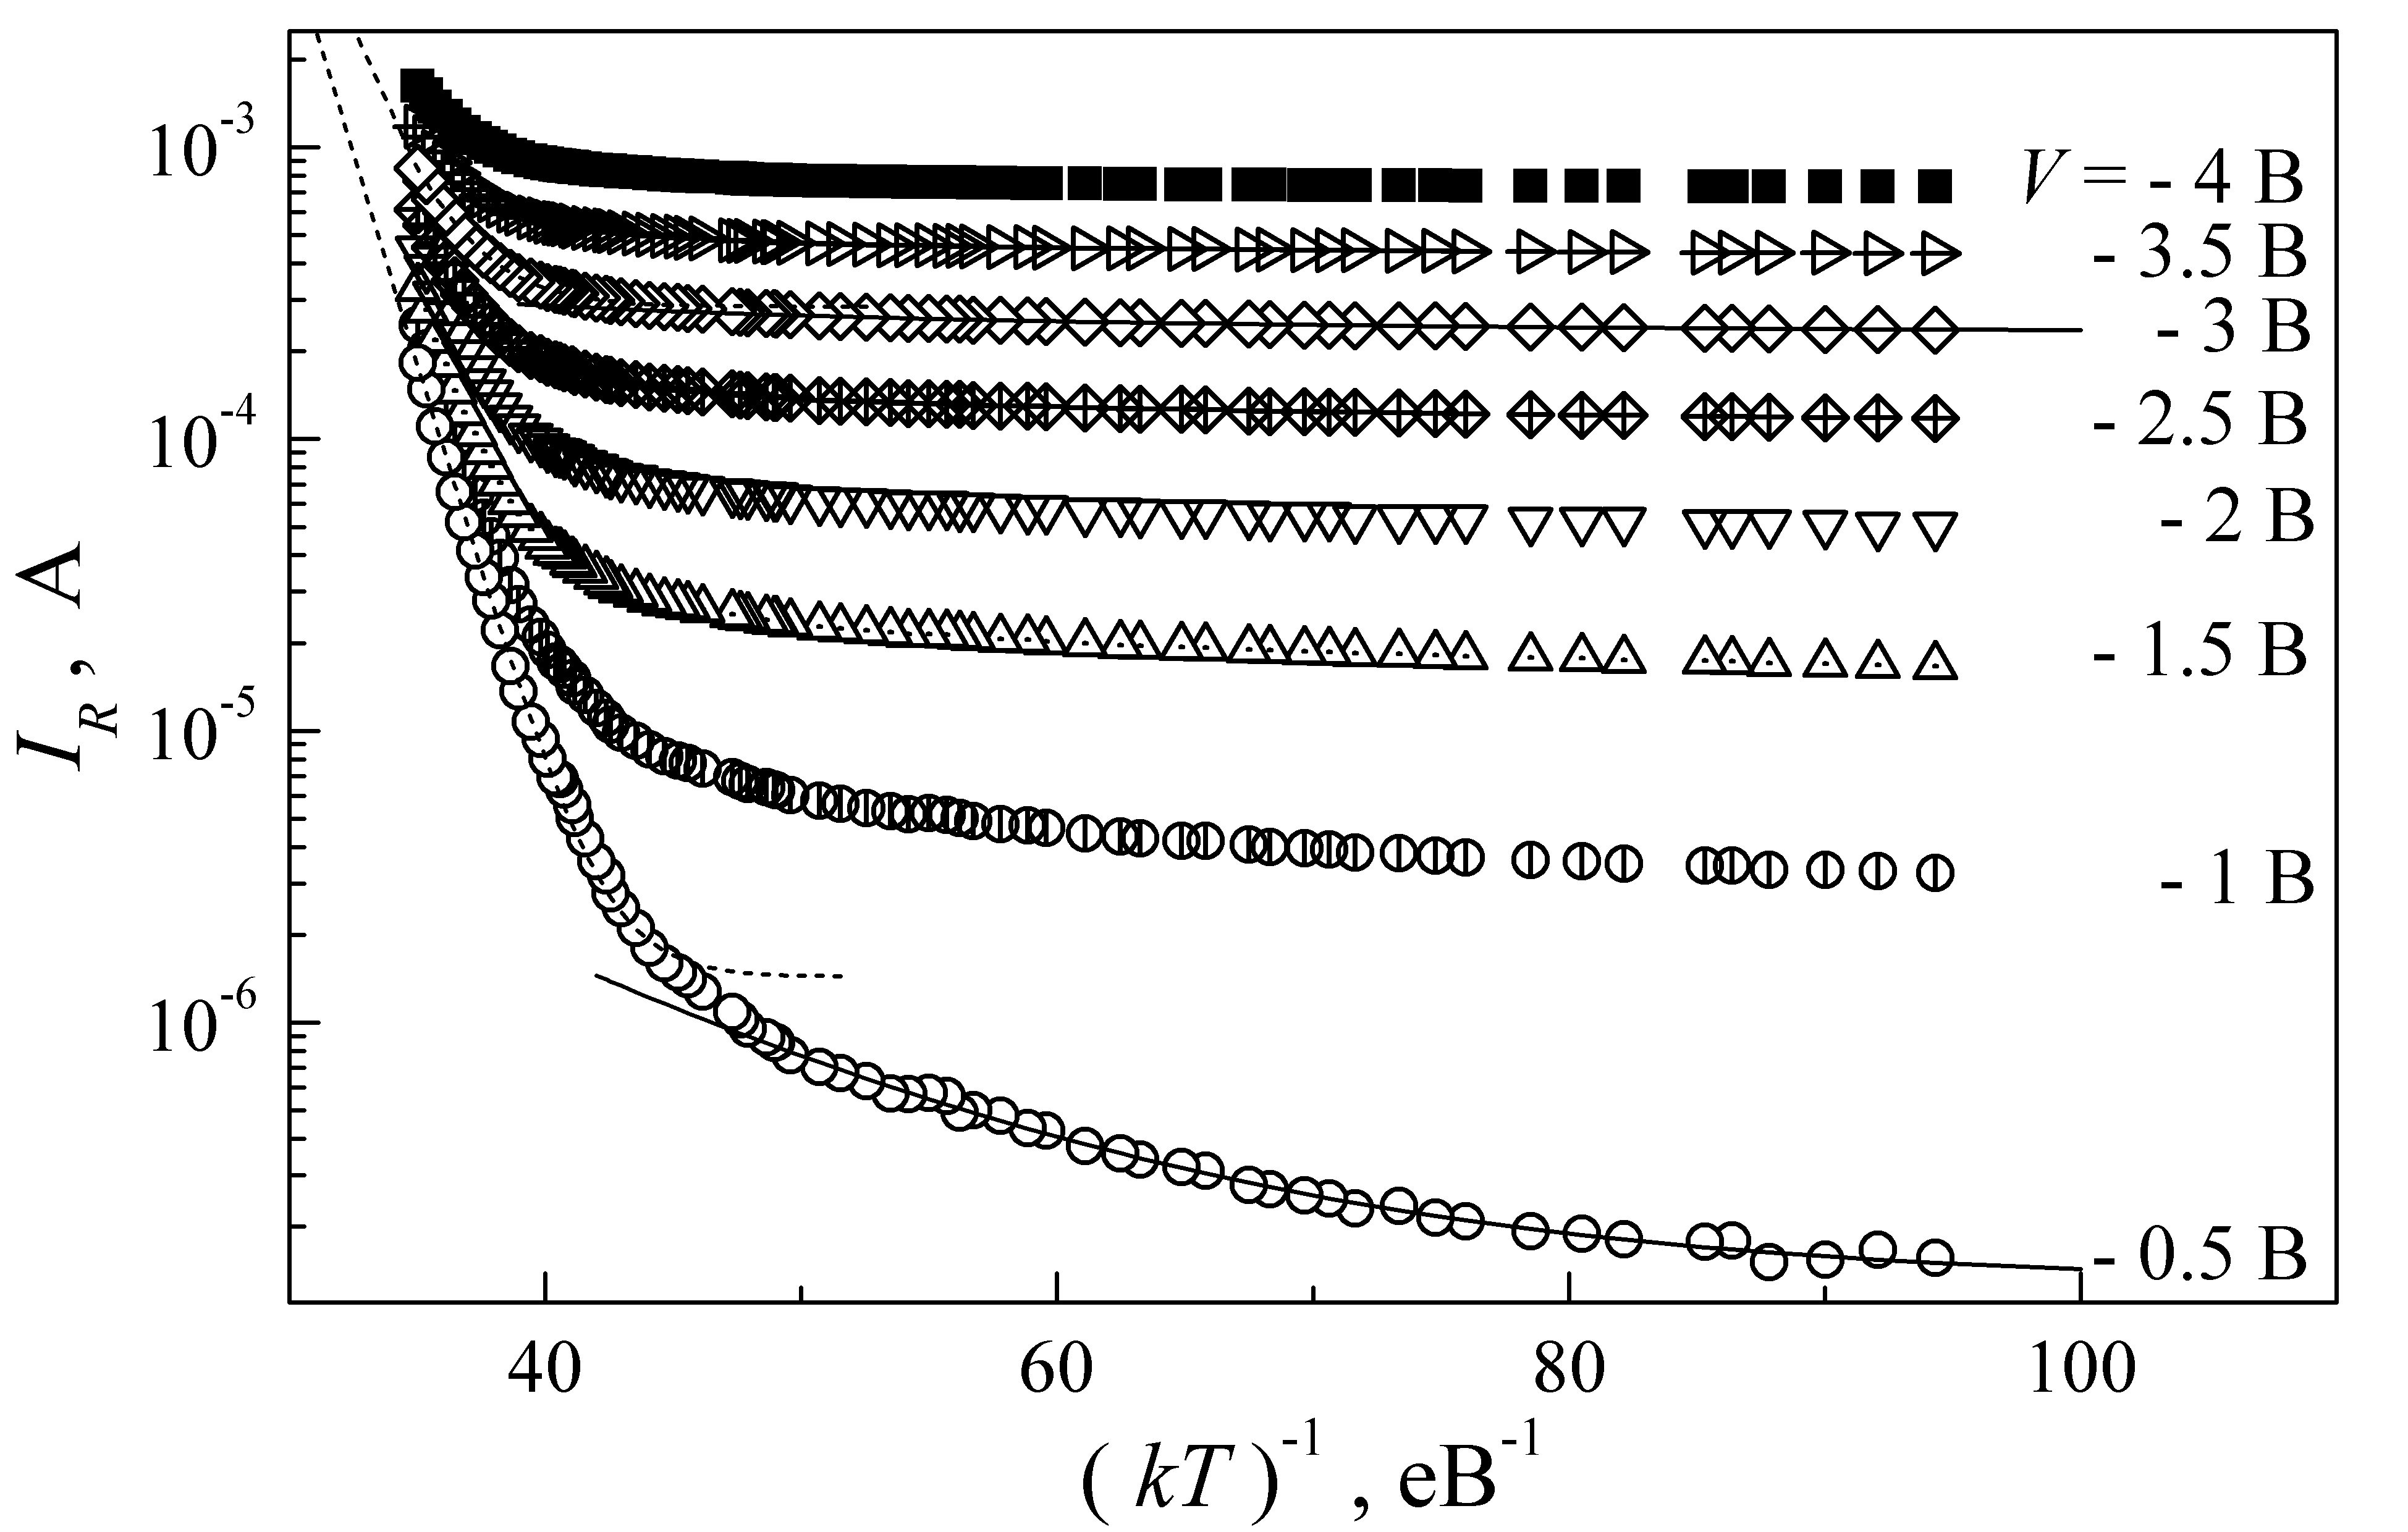
\includegraphics[width=0.7\textwidth]{figIT_SDAr}
\caption{\label{figIT_SDAr}
Температурна залежність зворотного струму структур SSDA при різних зміщеннях.
Точки --- експеримент, лінії --- апроксимація згідно з (\ref{eqIr})
(суцільні при $T=(130\div220)$~К, пунктирні при $T=(230\div330)$~К).
}%
\end{figure}

Проведений аналіз показав, що польова та температурна залежність зворотного струму можуть бути описані
за допомогою виразу
\begin{eqnarray}
\label{eqIr}
\nonumber I_R(T,V_R)&=&I_\mathrm{TE}(T,V_R)+I_\mathrm{FN}(V_R)=\\
&=&C_\mathrm{TE}(V_R)T^2\exp\left[-\frac{E_\mathrm{TE}(V_R)}{kT}\right]+I_\mathrm{FN}(V_R)\,,
\end{eqnarray}
де перший доданок $I_\mathrm{TE}$ описує ТЕ компоненту струму, яка залежить від температури та напруги,
а другий $I_\mathrm{FN}$ --- температурно-незалежну;
величини  $C_\mathrm{TE}$ та $E_\mathrm{TE}$ також не залежать від температури.

Для оцінки внеску кожної з компонент у загальний струм були використані величини
\begin{eqnarray*}
\nu_\mathrm{TE}&=&\frac{I_\mathrm{TE}}{I_R}=\frac{I_\mathrm{TE}}{I_\mathrm{TE}+I_\mathrm{FN}}\,,\\
\nu_\mathrm{FN}&=&\frac{I_\mathrm{FN}}{I_R}=\frac{I_\mathrm{FN}}{I_\mathrm{TE}+I_\mathrm{FN}}\,.
\end{eqnarray*}
Температурна та польова залежності $\nu_\mathrm{TE}$ та $\nu_\mathrm{FN}$ показані на Рис.~\ref{figeIr_SDA}.
Внесок ТЕ складової зростає при підвищенні температури та зменшенні зворотної напруги, проте характер
залежностей суттєво залежить від конкретних значень $T$ та $V_R$.


\begin{figure}
\center
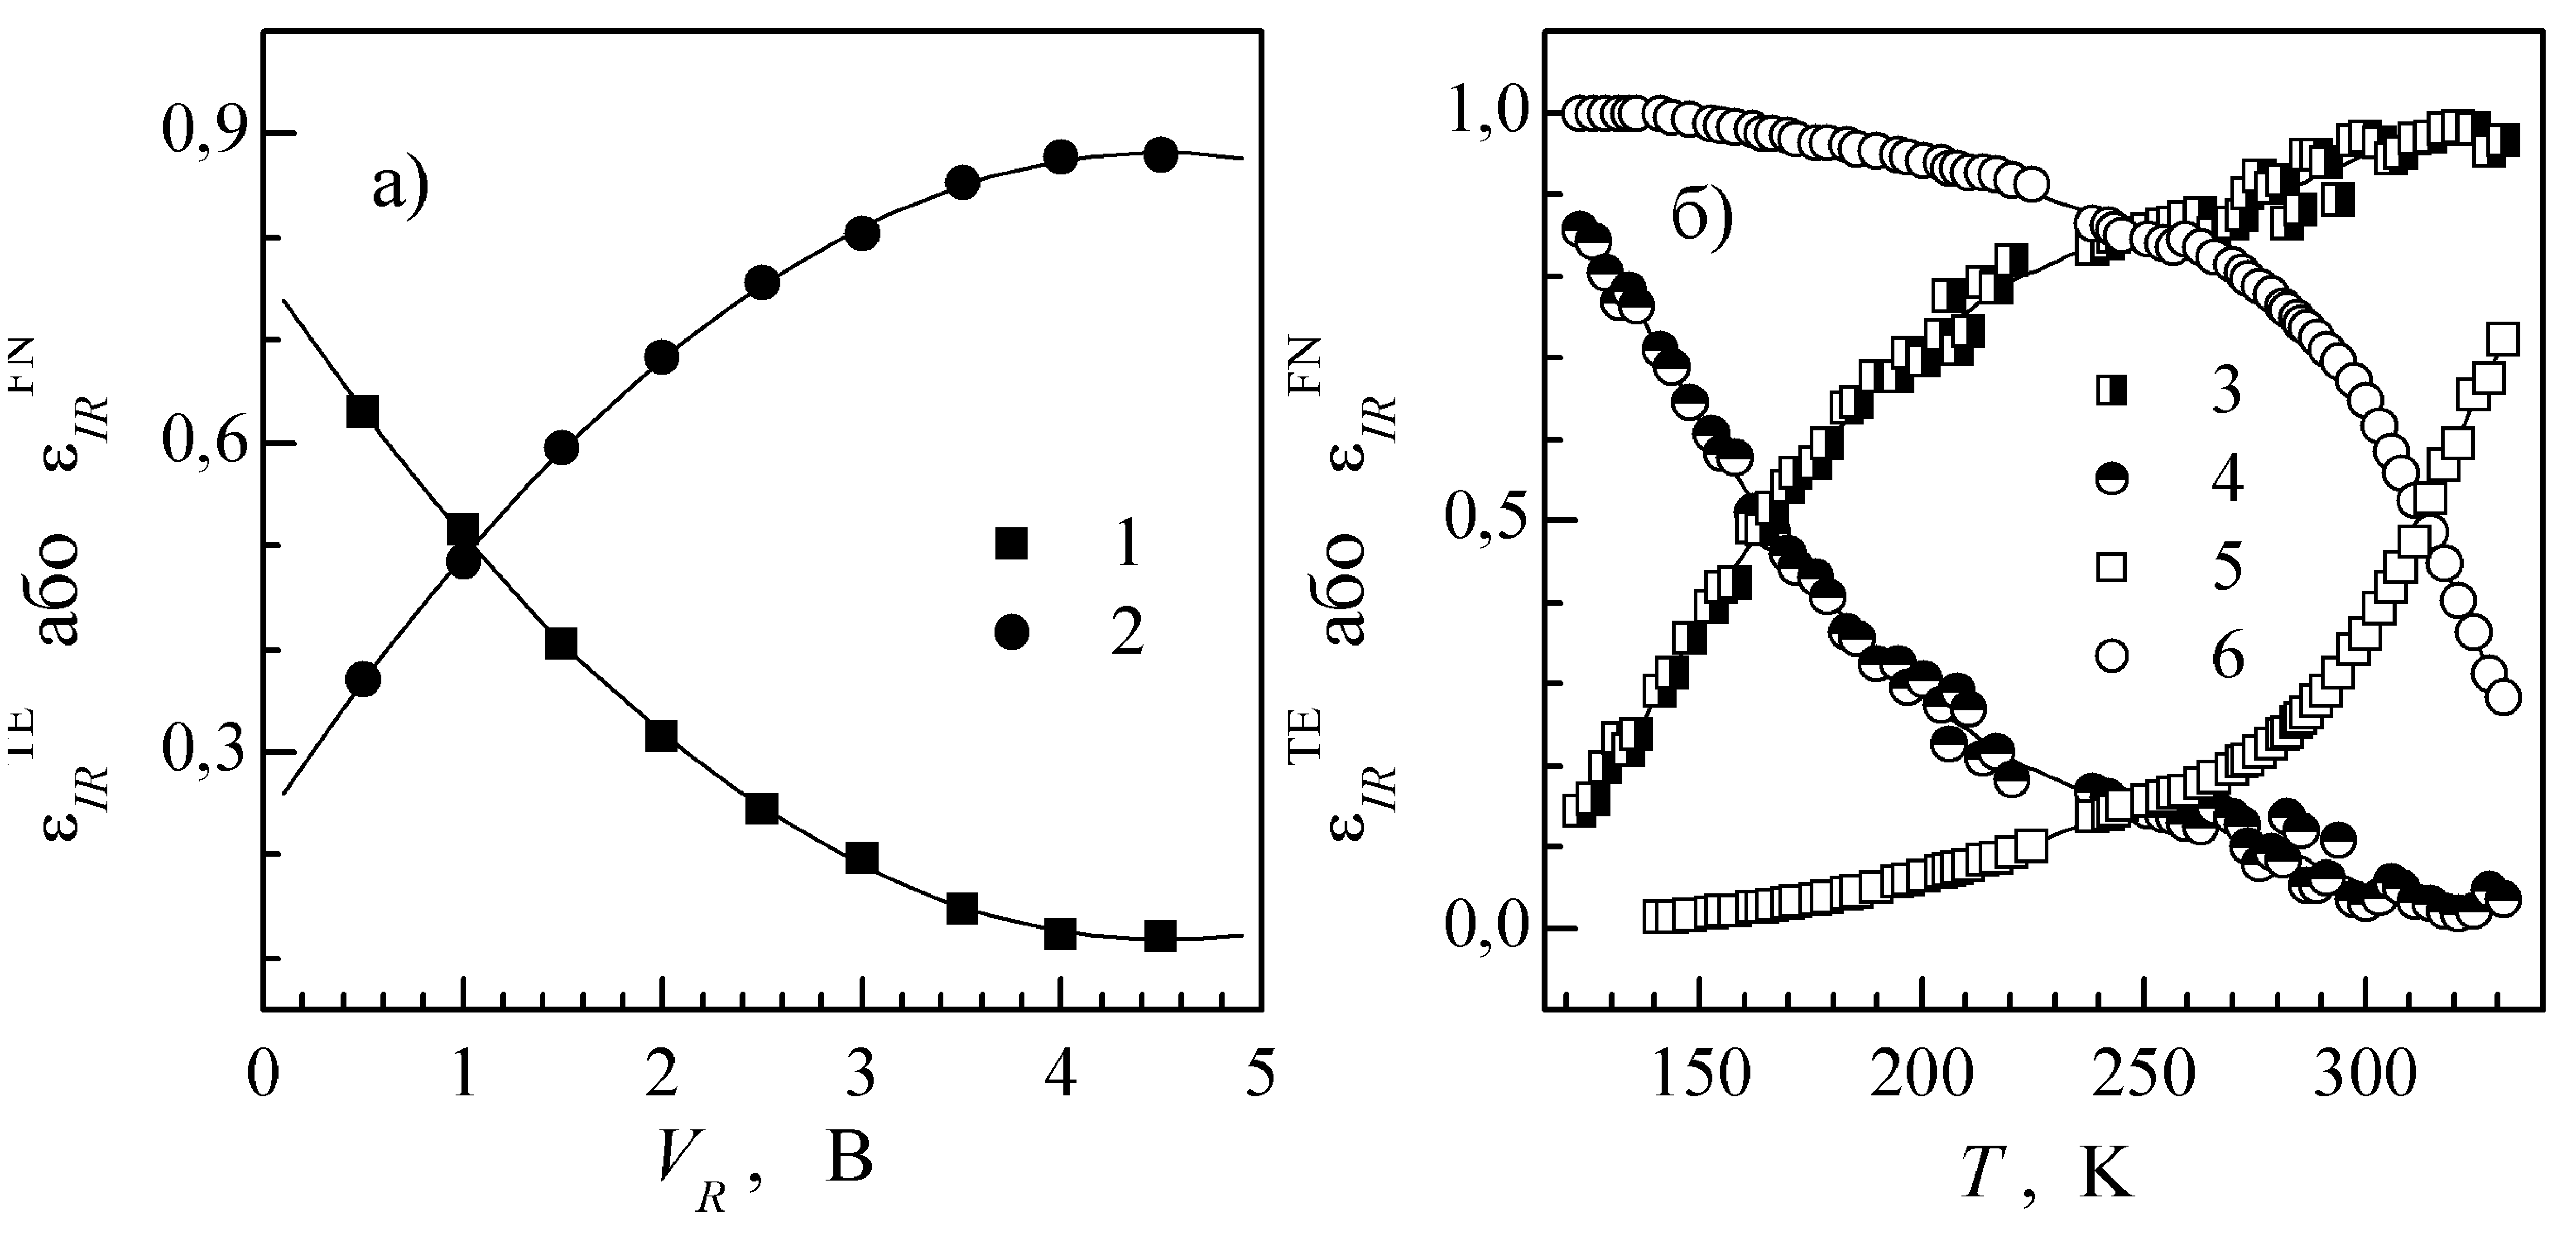
\includegraphics[width=0.8\textwidth]{figeIr_SDA}
\caption{\label{figeIr_SDA}
Залежність відносного внеску у зворотний струм
ТЕ (криві 1, 3 та 5) та температуро--незалежної (криві 2, 4 та 6)
компонент від зміщення при $T=300$~К (а) та
від температури (б) при $V_R=0,5$~В (3 та 4) і $V_R=3$~В (5 та 6).
}%
\end{figure}

Виявлена залежність характеристичної енергії $E_\mathrm{TE}$ від прикладеної напруги є свідченням зміни ВБШ.
Відомо \cite{Rhoderick1988,Tung:PhysRev,Andrews}, що зменшення висоти бар'єру при зворотному зміщенні може відбуватися під дією сил зображення
(при цьому  зміна ВБШ $\Delta\Phi_b\sim V_R^{1/4}$),
електричного поля ($\Delta\Phi_b\sim V_R^{1/2}$),
а також за рахунок впливу областей неоднорідності.
В останньому випадку $\Delta\Phi_b\sim V_R^{2/3}$, а коефіцієнт пропорційності залежить від параметрів цих локальних ділянок \cite{Tung:PhysRev}.
Для досліджених структур $E_\mathrm{TE}$ набуває різних значень в кожному з температурних піддіапазонів,
проте при збільшенні зворотного зміщення в обох випадках зменшується, лінійно спадаючи з зростанням $V^{2/3}$ --- див. Рис.~\ref{figIrTE_SDA}.
Таким чином, аналіз зворотних ВАХ також підтверджує,
що струм через досліджувані структури може бути описаний в рамках теорії неоднорідного контакту з патчами,
вплив яких на зарядоперенесення змінюється поблизу температури 225~К.



\begin{figure}
\center
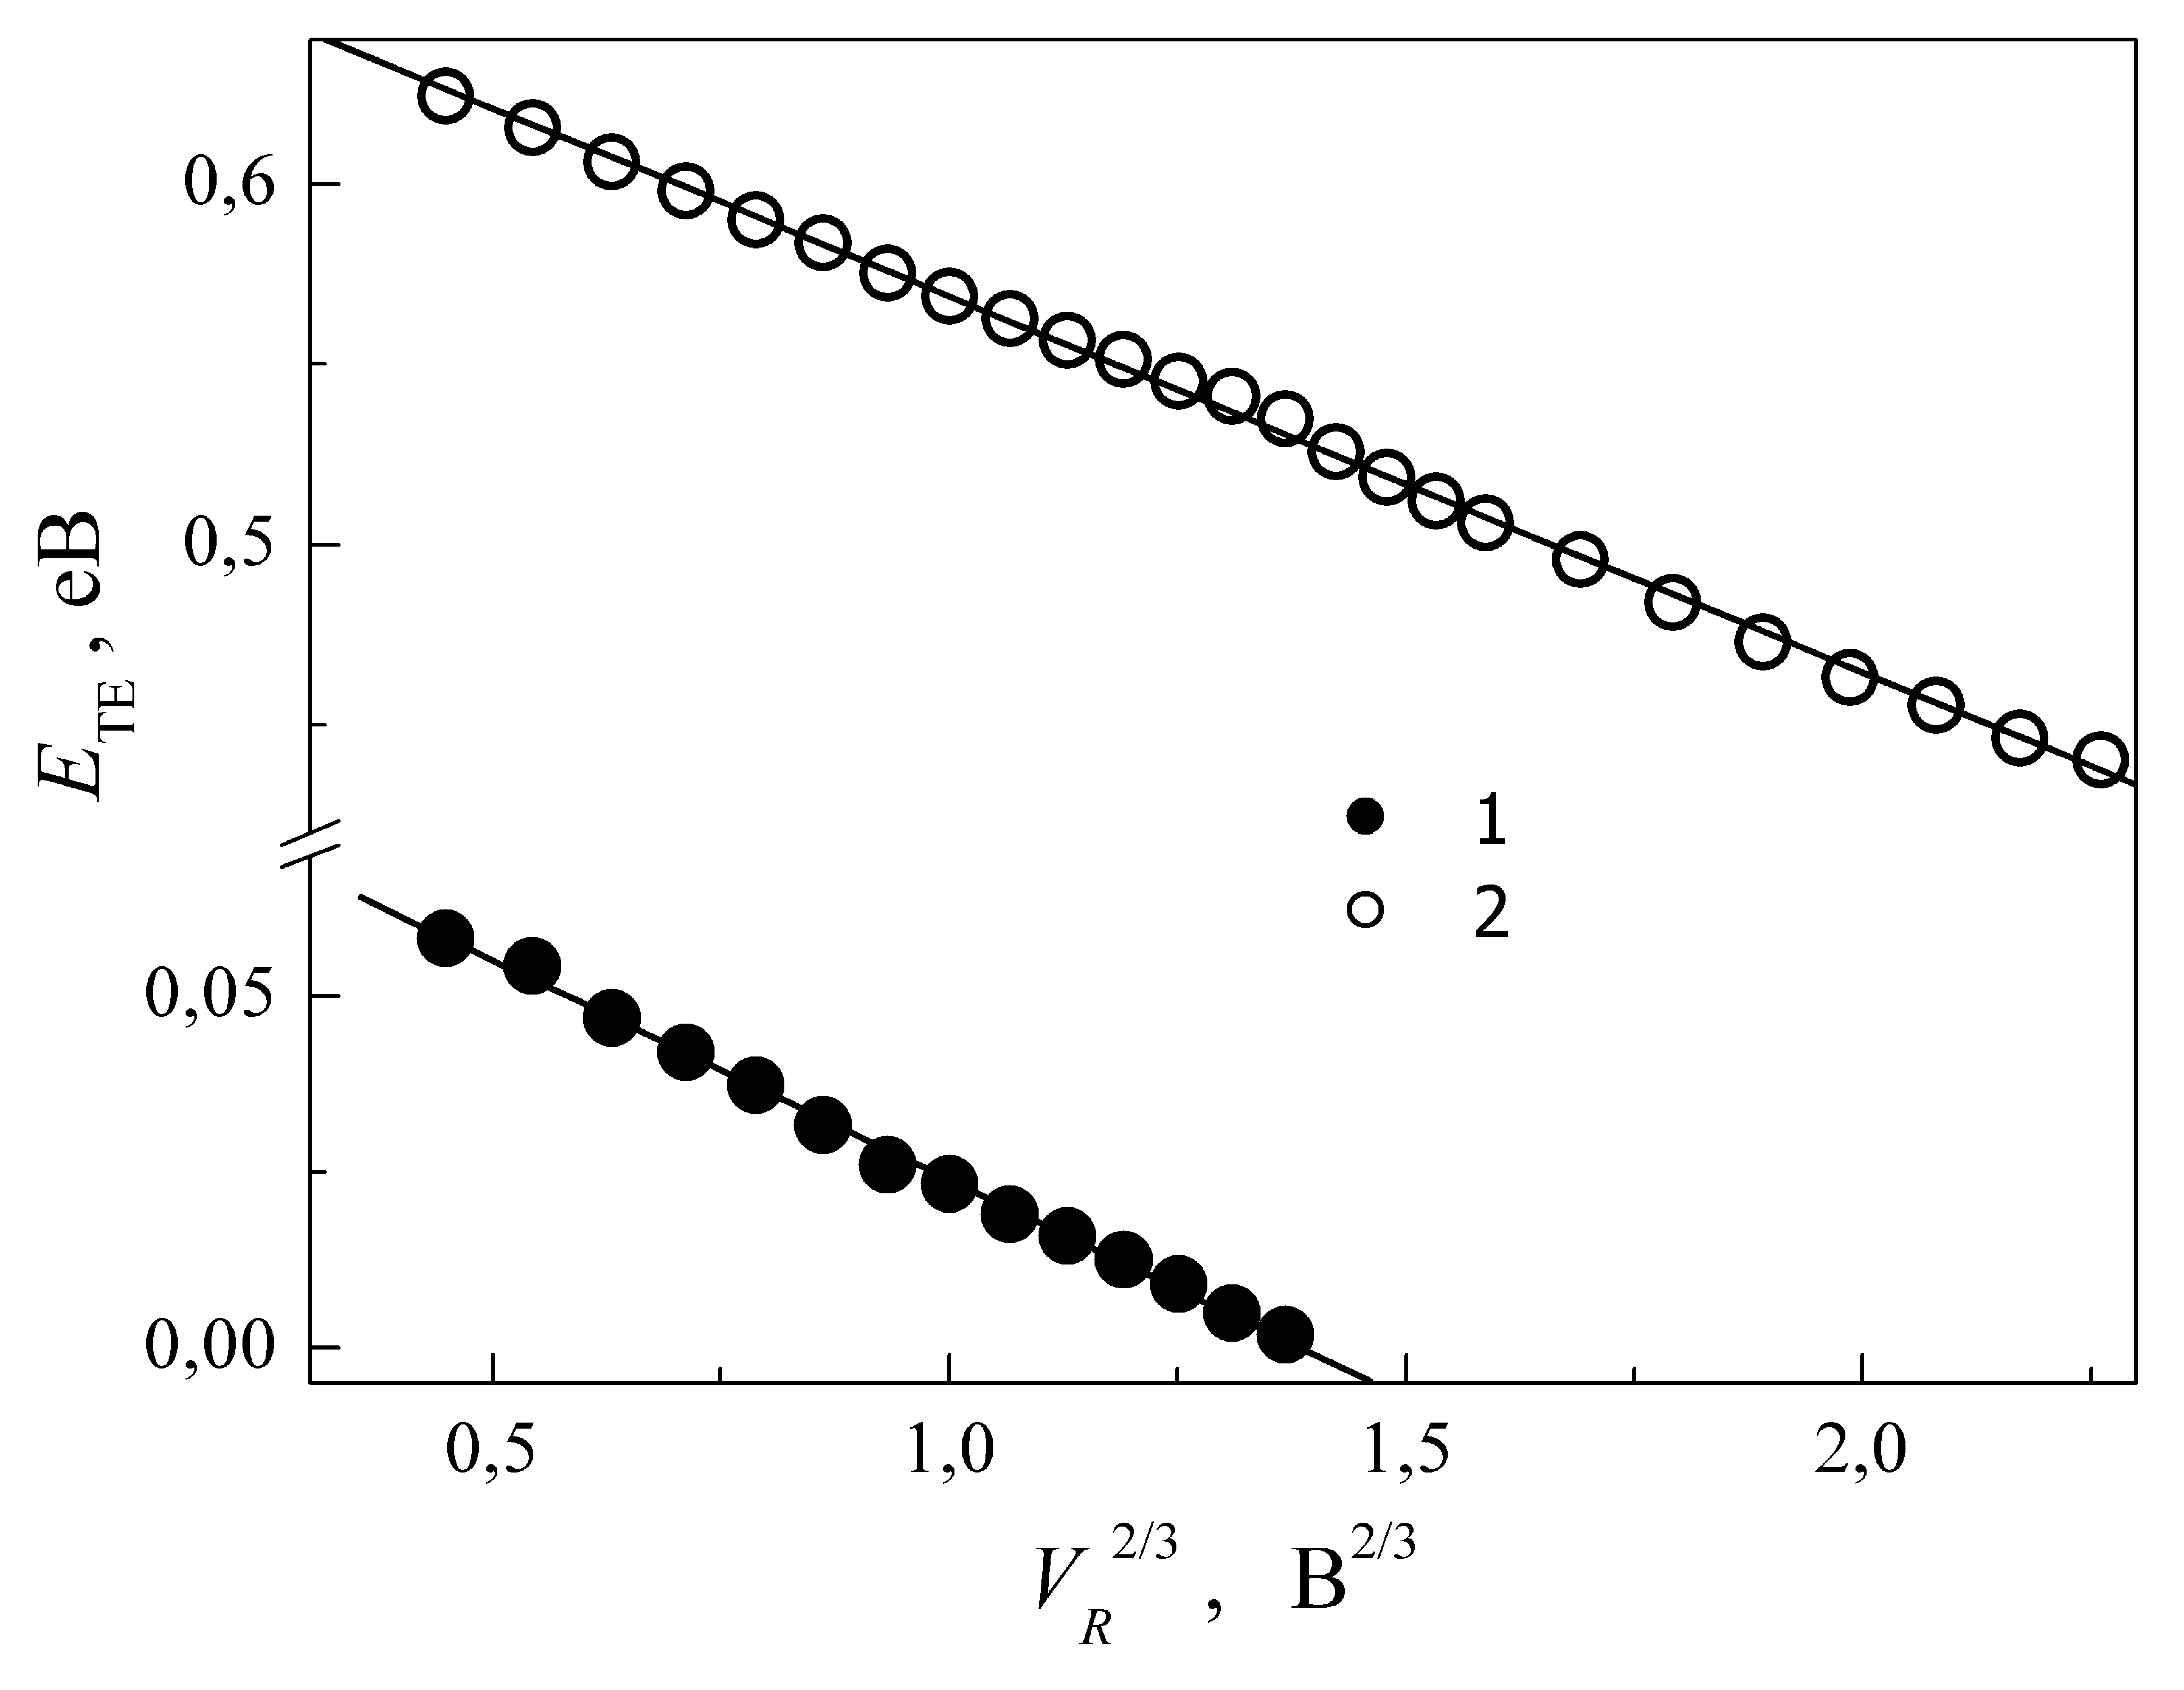
\includegraphics[width=0.65\textwidth]{figIrTE_SDA}
\caption{\label{figIrTE_SDA}
Польові залежності характеристичної енергії ТЕ складової зворотного струму
в діапазонах температур  $(130\div220)$~К (крива 1) та   $(230\div330)$~К (крива 2).
Точки --- експеримент, прямі --- лінійна апроксимація за методом найменших квадратів.
}%
\end{figure}

На Рис.~\ref{figIrFN_SDA} наведено польові залежності величини струму $I_\mathrm{FN}$ в координатах Фаулера--Нордгейма
$\ln(I_\mathrm{FN}/F_m^2)=f(1/F_M)$,
де
\begin{equation}\label{eqFm}
  F_m=\left(\frac{2qN_{d}V_{bb}}{\varepsilon_s\varepsilon_0}\right)^{1/2}
\end{equation}
напруженість електричного поля на границі розділу метал-напівпровідник \cite{Rhoderick1988};
при розрахунках $F_m$ використовувалися отримані при аналізі прямих ВАХ значення $\Phi^0_b$ та  $V_n$ при $T=250$~К.
Лінійність залежності свідчить про тунельний характер другої компоненти струму \cite{Evtuh},
що також підтверджується незалежністю величини $I_\mathrm{FN}$ від температури.


\begin{figure}
\center
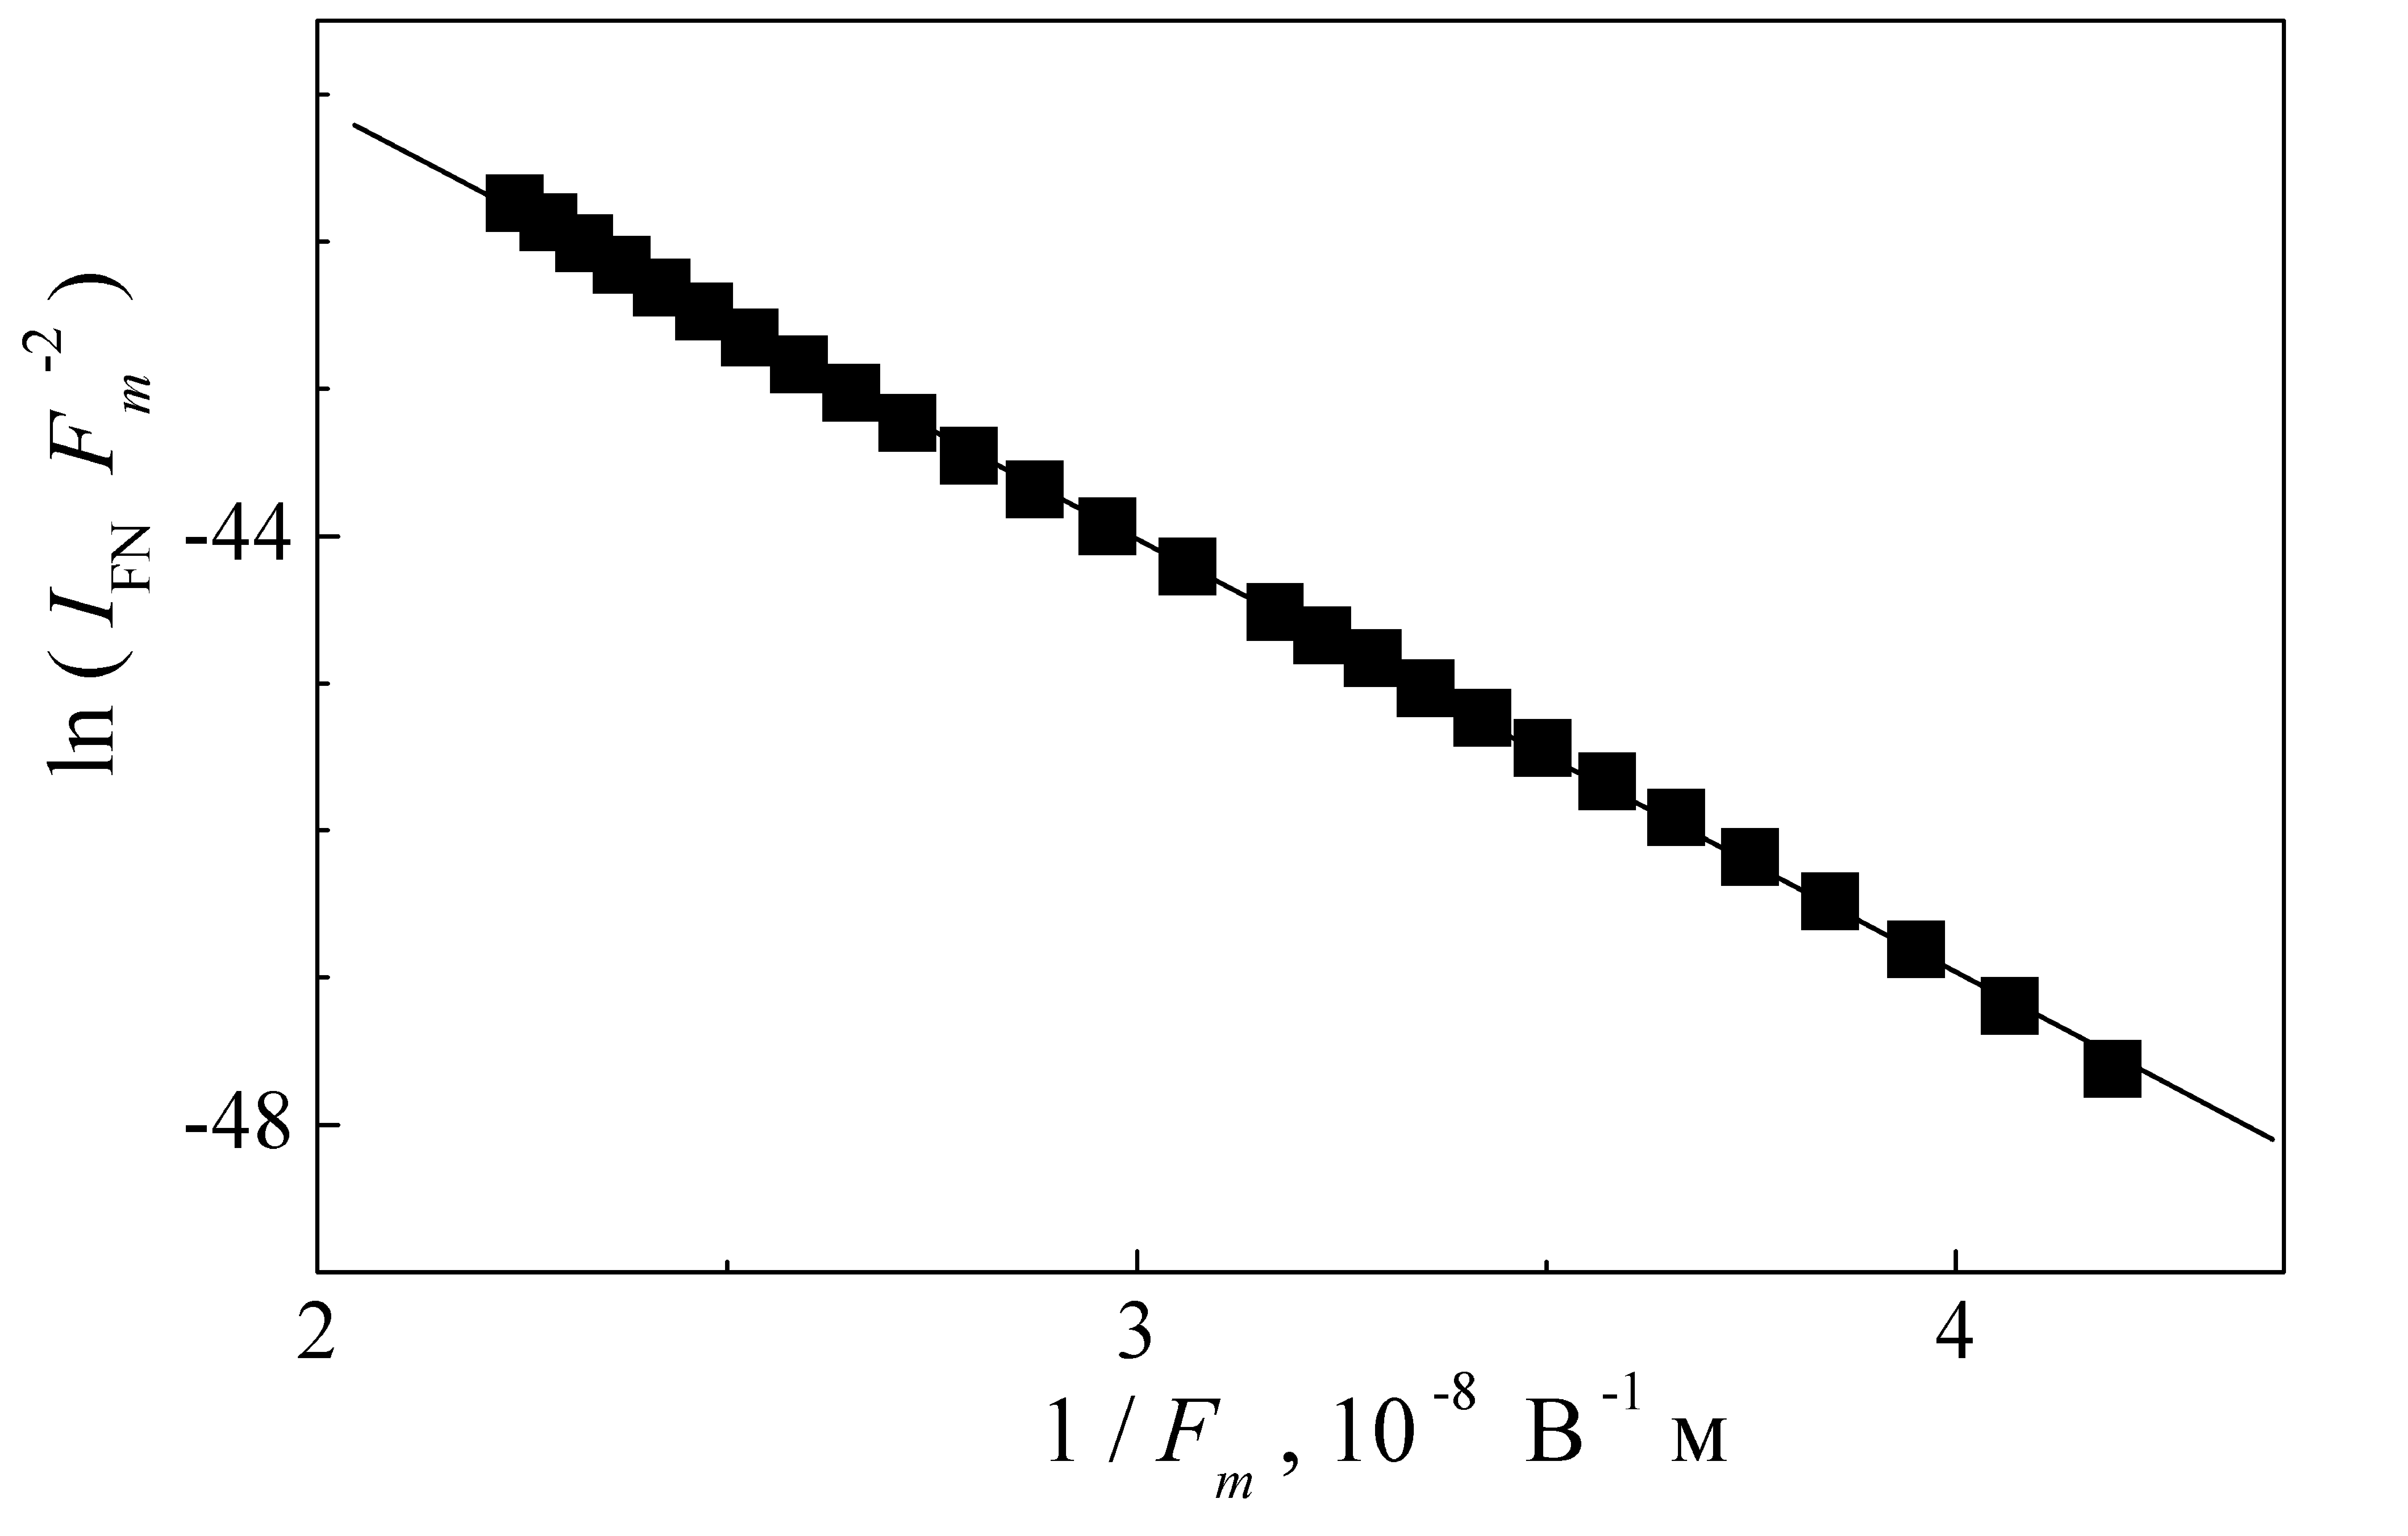
\includegraphics[width=0.65\textwidth]{figIrFN_SDA}
\caption{\label{figIrFN_SDA}
Залежність температуро--незалежної компоненти зворотного струму
в координатах Фаулера--Нордгейма.
Точки --- експеримент, пряма --- лінійна апроксимація за методом найменших квадратів.
}%
\end{figure}

Якщо тунелювання відбувається через трикутний бар'єр, то для опису струму може бути застосована
модифікована формула Фаулера--Нордгейма  \cite{Rhoderick1988,Novikov,Kurnosova}:
\begin{equation}\label{eqFowlNord}
    \ln\left(\frac{I_\mathrm{FN}}{F_m^2}\right)\propto -\frac{4 \sqrt{2m^*}(qE_{t,\mathrm{eff}})^{3/2}}{3\hbar q F_m}\,,
\end{equation}
де
$m*$ ---  ефективна маса електрону,
для Si $m* = 1,08\cdot9,11\cdot10^{-31}$~кг,
$E_{t,\mathrm{eff}}$ --– ефективна енергія тунелювання,
яка для випадку тунелюванням через центр у забороненій зоні залежить від глибини залягання рівня $E_a=E_c-E_t$ \cite{Kurnosova,Bulyarskii2001r}:
\begin{equation}\label{eqFN:Et}
    E_{t,\mathrm{eff}}=E_g\left\{\frac{3}{16}\left[\frac{\pi}{2}-
     \arcsin\left(1-\frac{2E_a}{E_g}\right)\right]-\frac{3}{8}\left(1-\frac{2E_a}{E_g}\right)
     \sqrt{\frac{E_a}{E_g}-\left(\frac{E_a}{E_g}\right)^2}\right\}^{2/3}
\end{equation}


Апроксимуючи отриману залежність (Рис.~\ref{figIrFN_SDA}) згідно з (\ref{eqFowlNord}) та використовуючи (\ref{eqFN:Et}),
знайдено, $E_c-E_t=(120\pm5)$~меВ.
Ця величина добре узгоджується з акцепторним рівнем міжвузольного атому вуглецю С$i$ $E_c-(0,10\div0,12)$~еВ \cite{Vavilov1990r,Song1987}.
Таким чином, струм $I_\mathrm{FN}$ добре описується моделлю прямого тунелюванням через глибокий центр, яким, імовірно, є міжвузольний атом вуглецю.
